\documentclass[11pt,usenames]{article}
\usepackage{srcltx,pdfsync}
%\usepackage[pdflatex=false,recompilepics]{gastex} 
\usepackage{amsmath,amssymb,amsfonts}
\usepackage{color}
\usepackage{hyperref, url}
\usepackage{geometry}
\usepackage{graphicx,subfigure,wrapfig}
\geometry{verbose,a4paper,tmargin=30mm,bmargin=50 mm,lmargin=25mm,rmargin=16mm}
\usepackage{ifthen}

\def\Lap{\ensuremath{\mathcal{L}}}
\usepackage{fancyhdr}
\pdfpagewidth 8.5in
\pdfpageheight 11in

\pagestyle{fancy}
\headheight 35pt

\usepackage{listings}
\usepackage{color} %red, green, blue, yellow, cyan, magenta, black, white
\definecolor{mygreen}{RGB}{28,172,0} % color values Red, Green, Blue
\definecolor{mylilas}{RGB}{170,55,241}


\graphicspath{{./Images}}

%%%%%%%%%%%%%
\usepackage[fancythm]{jphmacros2e}
\renewcommand{\footrulewidth}{0.5 pt}

\rhead{\small{Project Report}}
\chead{}
\lhead{\small{EML 6934}}
\lfoot{Ninad Gaikwad}
\cfoot{\thepage}
\rfoot{}

\title{}

\date{}
\begin{document}
	
	
	\lstset{language=Matlab,%
		%basicstyle=\color{red},
		breaklines=true,%
		morekeywords={matlab2tikz},
		keywordstyle=\color{blue},%
		morekeywords=[2]{1}, keywordstyle=[2]{\color{black}},
		identifierstyle=\color{black},%
		stringstyle=\color{mylilas},
		commentstyle=\color{mygreen},%
		showstringspaces=false,%without this there will be a symbol in the places where there is a space
		numbers=left,%
		numberstyle={\tiny \color{black}},% size of the numbers
		numbersep=9pt, % this defines how far the numbers are from the text
		emph=[1]{for,end,break},emphstyle=[1]\color{red}, %some words to emphasise
		%emph=[2]{word1,word2}, emphstyle=[2]{style},    
	}
	
	\begin{center}
		{\sc Optimal Control}\\
		University of Florida \\
		Mechanical and Aerospace Engineering
		\vspace{0.5 cm}
	\end{center}
	
	{\large \begin{center}
			\textbf{Project - Report}\\
			Optimal Control Indirect and Direct Method Implementation
	\end{center}}
	
	
	\newpage
	
	
	\tableofcontents
	
	
	\newpage
	
	
	\section{Elementary Problem: Linear Tangent Steering}
	
	
	\subsection{Problem Formulation:}
	
	The Linear Tangent Steering Optimal Control Problem is as follows;\\
	
	Minimize the cost functional,
	
	\begin{align} 
	J = t_{f},
	\end{align}
	
	Subject to the dynamic constraints,
	
	\begin{align}
	\dot x_{1} &= x_{3}, \nonumber \\
	\dot x_{2} &= x_{4},\\
	\dot x_{3} &= a.cos(u),\nonumber\\
	\dot x_{4} &= a.sin(u), \nonumber
	\end{align}
	
	With the following boundary conditions,
	
	\begin{align}
	t_{0} &= 0 & t_{f} &= \text{Free}, \nonumber \\
	x_{1}(0) &= 0 & x_{1}(t_{f}) &= \text{Free}, \nonumber \\
	x_{2}(0) &= 0 & x_{2}(t_{f}) &= 5, \\
	x_{3}(0) &= 0 & x_{3}(t_{f}) &= 45, \nonumber \\
	x_{4}(0) &= 0 & x_{4}(t_{f}) &= 0, \nonumber 
	\end{align}
	
	Where $a=100$.
	
	\newpage
	
	
	\subsection{Indirect Method: Hamiltonian Boundary Value Problem [HBVP]}
	\subsubsection{Optimal Solution: Using Optimal Control Theory}
	
	We have,
	
	\begin{align}
	J &= t_{f} , \nonumber  
	\end{align}
	
	We know,
	
	\begin{align}
	J &= M + \int_{t_{0}}^{t_{f}} L \text{   } dt ,  \nonumber 
	\end{align}
	
	Where,
	
	\begin{align}
	M &= \text{Meyer Cost} \nonumber \\
	L &= \text{Lagrange Cost} \nonumber
	\end{align}
	
	Now we know that,
	
	\begin{align}
	M &= t_{f}, \nonumber \\
	L &= 0, \nonumber
	\end{align}
	
	Creating the Hamiltonian,
	
	\begin{align}
	H = L + \underbar{\lambda^{T}} \underbar{f},
	\end{align}
	
	Where,
	
	\begin{align}
	L &= 0, \nonumber \\
	\underbar \lambda^{T} &= \left[  \lambda_{x_{1}} \quad \lambda_{x_{2}} \quad \lambda_{x_{3}} \quad \lambda_{x_{4}}  \right],  \\
	\underbar f &=
	\begin{bmatrix}
	x_{3} \\ \ x_{4} \\  a.cos(u) \\ \ a.sin(u) 
	\end{bmatrix}, \nonumber 
	\end{align}
	
	
	\newpage
	
	
	Hence the Hamiltonian is as follows,
	
	\begin{align}
	H = \lambda_{x_{1}} \left[  x_{3} \right] + \lambda_{x_{2}} \left[  x_{4} \right] + \lambda_{x_{3}} \left[  a.cos(u) \right] + \lambda_{x_{4}} \left[  a.sin(u) \right] ,
	\end{align}
	
	Now, using $ 1^{st} $ Order Optimality Conditions for $ \underbar x $, 
	
	\begin{align}
	\dot{\underbar x} &= \left[ \frac{\partial H}{\partial{\underbar \lambda}}  \right]^{T}  ,\\
	\end{align}
	
	We get,
	
	\begin{align}
	\dot x_{1} &= \frac{\partial H}{\partial \lambda_{x_{1}}}  &= x_{3}, \nonumber \\
	\dot x_{2} &= \frac{\partial H}{\partial \lambda_{x_{2}}}  &= x_{4},\\
	\dot x_{3} &= \frac{\partial H}{\partial \lambda_{x_{3}}}  &= a.cos(u),\nonumber\\
	\dot x_{4} &= \frac{\partial H}{\partial \lambda_{x_{4}}}  &= a.sin(u), \nonumber
	\end{align}
	
	Now, using $ 1^{st} $ Order Optimality Conditions for $  \underbar\lambda $, 
	
	\begin{align}
	\dot{\underbar \lambda} &= - \left[ \frac{\partial H}{\partial{\underbar x}}  \right]^{T}  ,
	\end{align}
	
	We get,
	
	\begin{align}
	\dot{\lambda_{x_{1}}} &= - \frac{\partial H}{\partial x_{1}}  &= 0, \nonumber \\
	\dot{\lambda_{x_{2}}} &= - \frac{\partial H}{\partial x_{2}}  &= 0,\\
	\dot{\lambda_{x_{3}}} &= - \frac{\partial H}{\partial x_{3}}  &= - \lambda_{x_{1}},\nonumber\\
	\dot{\lambda_{x_{4}}} &= - \frac{\partial H}{\partial x_{4}}  &= - \lambda_{x_{2}}, \nonumber
	\end{align}
	
	
	\newpage
	
	
	Now, using $ 1^{st} $ Order Optimality Conditions for $ H $, 
	
	\begin{align}
	\left[ \frac{\partial H}{\partial u}  \right] &= 0  ,
	\end{align}
	
	We get,
	
	\begin{align}
	\left[ \frac{\partial H}{\partial u}  \right] &= -a.\lambda_{x_{3}}.sin(u) + a.\lambda_{x_{4}}.cos(u)  , \nonumber \\
	\frac{\lambda_{x_{4}}}{\lambda_{x_{3}}}  &= tan(u) , \nonumber
	\end{align}
	
	Therefore, we have,
	
	\begin{align}
	u &= tan^{-1} \left[ \frac{\lambda_{x_{4}}}{\lambda_{x_{3}}} , \right]
	\end{align}
	
	Since $\delta t_{f}$ and $\delta \underbar{x}_{f}$ are not fixed, we can use the following Transversality Conditions,
	
	\begin{align}
	\left[ \frac{\partial M}{\partial{\underbar{x}(t_{f})} } - \nu^{T} \frac{\partial \underbar b}{\partial{\underbar{x}(t_{f})} } - \underbar{\lambda^{T}}(t_{f}) \right]&= \underbar 0^{T} \\
	\left[ \frac{\partial M}{\partial{t_{f}} } - \nu^{T} \frac{\partial \underbar b}{\partial{t_{f}} } + H(t_{f}) \right]&=  0 ,
	\end{align}
	
	Where,
	
	\begin{align}
	\underbar b &= 
	\begin{bmatrix}
	x_{1}(t_{0})-0 \\ x_{2}(t_{0})-0 \\ x_{3}(t_{0})-0 \\ x_{4}(t_{0})-0 \\ x_{2}(t_{f})-5 \\ x_{3}(t_{f})-45 \\ x_{4}(t_{f})-0 \\
	\end{bmatrix} , \nonumber
	\end{align}
	
	and,
	
	\begin{align}
	\underbar{\nu^{T}} &= \left[ \nu_{1} \quad \nu_{2} \quad \nu_{3} \quad \nu_{4} \quad \nu_{5} \quad \nu_{6} \quad \nu_{7} \right] , \nonumber
	\end{align}
	
	
	\newpage
	
	
	Computing terms for the Transversality condition corresponding to $\delta \underbar{x}_{f} \neq 0$ , we get,
	
	\begin{align}
	\frac{\partial M}{\partial{ \underbar{x}_{t_{f}}}} &= \left[ \quad \frac{\partial M}{\partial{x_{1}(t_{f})}}  \quad \frac{\partial M}{\partial{x_{2}(t_{f})}} \quad \frac{\partial M}{\partial{x_{3}(t_{f})}} \quad \frac{\partial M}{\partial{x_{4}(t_{f})}} \quad \right], \nonumber \\
	\frac{\partial M}{\partial{ \underbar{x}_{t_{f}}}} &= \left[ \quad \frac{\partial t_{f}}{\partial{x_{1}(t_{f})}}  \quad \frac{\partial t_{f}}{\partial{x_{2}(t_{f})}} \quad \frac{\partial t_{f}}{\partial{x_{3}(t_{f})}} \quad \frac{\partial t_{f}}{\partial{x_{4}(t_{f})}} \quad \right], \nonumber \\
	\frac{\partial M}{\partial{ \underbar{x}_{t_{f}}}} &= \left[ \quad 0 \quad 0  \quad 0  \quad 0 \quad  \right],
	\end{align}
	
	\begin{align}
	\frac{\partial{\underbar b}}{\partial{ \underbar{x}_{t_{f}}}} &= \left[ \quad \frac{\partial{\underbar b}}{\partial{x_{1}(t_{f})}} \quad \frac{\partial{\underbar b}}{\partial{x_{2}(t_{f})}} \quad \frac{\partial{\underbar b}}{\partial{x_{3}(t_{f})}} \quad \frac{\partial{\underbar b}}{\partial{x_{4}(t_{f})}}  \quad \right], \nonumber \\
	\frac{\partial{\underbar b}}{\partial{ \underbar{x}_{t_{f}}}} &=
	\begin{bmatrix}
	0 \quad 0 \quad 0 \quad 0 \\ 0 \quad 0 \quad 0 \quad 0  \\ 0 \quad 0 \quad 0 \quad 0  \\ 0 \quad 0 \quad 0 \quad 0  \\ 0 \quad 1 \quad 0 \quad 0  \\ 0 \quad 0 \quad 1 \quad 0  \\ 0 \quad 0 \quad 0 \quad 1  \\
	\end{bmatrix} , \\
	\nu^{T} \frac{\partial \underbar b}{\partial{\underbar{x}(t_{f})} } &= \left[ \quad 0 \quad \nu_{5} \quad \nu_{6} \quad \nu_{7} \quad \right],
	\end{align}
	
	Now, we have,
	
	\begin{align}
	\left[ \frac{\partial M}{\partial{\underbar{x}(t_{f})} } - \nu^{T} \frac{\partial \underbar b}{\partial{\underbar{x}(t_{f})} } - \underbar{\lambda^{T}}(t_{f}) \right]&= \underbar 0^{T} \nonumber \\
	\left[ \quad 0 \quad 0 \quad 0 \quad 0 \quad  \right] - \left[ \quad 0 \quad \nu_{5} \quad \nu_{6} \quad \nu_{7} \quad \right] - \left[ \quad \lambda_{x_{1}}(t_{f}) \quad \lambda_{x_{2}}(t_{f}) \quad \lambda_{x_{3}}(t_{f}) \quad \lambda_{x_{4}}(t_{f}) \quad \right] &= \underbar 0^{T} \nonumber 
	\end{align}
	
	Therefore, we get,
	
	\begin{align}
	\lambda_{x_{1}}(t_{f}) &= 0, 
	\end{align}
	
	and from equations (11) and (19) we have,
	\begin{align}
	\lambda_{x_{1}}(t_{0}) &= 0, 
	\end{align}
	
	
	\newpage
	
	
	Computing terms for the Transversality condition corresponding to $\delta t_{f} \neq 0$, we get,
	
	\begin{align}
	\frac{\partial{\underbar M}}{\partial{ t_{f}}} &= \left[ \quad \frac{\partial t_{f}}{\partial{x_{1}(t_{f})}}  \quad  \right] &= 1 ,  \\
	\frac{\partial b}{\partial{ t_{f}}} &= 
	\begin{bmatrix}
	0 \\ 0 \\ 0 \\ 0 \\ 0 \\ 0 \\ 0 \\
	\end{bmatrix},  \\
	\nu^{T} \frac{\partial \underbar b}{\partial{\underbar{x}(t_{f})} } &= 0,
	\end{align}
	
	Now, we have,
	
	\begin{align}
	\left[ \frac{\partial M}{\partial{\underbar{x}(t_{f})} } - \nu^{T} \frac{\partial \underbar b}{\partial{\underbar{x}(t_{f})} } + H(t_{f}) \right]&=  0 \nonumber \\
	\left[ \quad 1 \quad  \right] - \left[ \quad 0 \quad  \right] + \left[ \quad H(t_{f}) \quad \right] &=  0 \nonumber 
	\end{align}
	
	Therefore, we get,
	
	\begin{align}
	H(t_{f}) &= -1, 
	\end{align}
	
	
	\newpage
	
	
	Formulating the HBVP,
	
	
	
	Known Initial Conditions are as follows,
	
	\begin{align}
	x_{1}(0) &= 0 , \nonumber \\
	x_{2}(0) &= 0 , \nonumber \\
	x_{3}(0) &= 0 ,  \\
	x_{4}(0) &= 0 , \nonumber \\
	\lambda_{x_{1}}(0) &= 0 , \nonumber \\
	t_{0} &= 0 , \nonumber \\
	\end{align}
	
	
	
	Unknown Initial Conditions are as follows,
	
	\begin{align}
	\lambda_{x_{2}}(0) &= \text{??} , \nonumber \\
	\lambda_{x_{3}}(0) &= \text{??} ,  \\
	\lambda_{x_{4}}(0) &= \text{??} , \nonumber \\
	t_{f} &= 0 , \nonumber \\
	\end{align}
	
	Note:
	\begin{itemize}
		\item The Root Finder has to find the Optimal Values for these variables.
		\item We need to provide an initial guess for these variables.
	\end{itemize}
	
	Dynamics to be integrated,
	
	\begin{align}
	\dot x_{1}(t) &= x_{3}(t), \nonumber \\
	\dot x_{2}(t) &= x_{4}(t), \nonumber \\
	\dot x_{3}(t) &= a.cos(u(t)),\nonumber\\
	\dot x_{4}(t) &= a.sin(u(t)),  \\
	\dot{\lambda_{x_{1}}}(t) &= 0, \nonumber \\
	\dot{\lambda_{x_{2}}}(t) &= 0, \nonumber \\
	\dot{\lambda_{x_{3}}}(t) &= - \lambda_{x_{1}}(t),\nonumber\\
	\dot{\lambda_{x_{4}}}(t) &= - \lambda_{x_{2}}(t), \nonumber
	\end{align}
	
	Where,
	
	\begin{align}
	u &= tan^{-1} \left[ \frac{\lambda_{x_{4}}}{\lambda_{x_{3}}} , \right]
	\end{align}
	
	Error to be minimized to zero is as follows,
	
	\begin{align}
	\underbar e &= 
	\begin{bmatrix}
	x_{2}(t_{f})-5 \\ x_{3}(t_{f})-45 \\ x_{4}(t_{f})-0 \\ \lambda_{x_{1}}(t_{f})-0 \\ H(t_{f})+1 \\ 
	\end{bmatrix} 
	&= 
	\begin{bmatrix}
	0 \\ 0 \\ 0 \\ 0 \\ 0
	\end{bmatrix} 
	\end{align}
	
	
	
	\newpage
	
	
	\subsubsection{MATLAB Code}
	
	\lstinputlisting{LinearTangent_Main.m}
	
	\newpage
	
	\lstinputlisting{LinearTangent_ODEEquations.m}
	
	\newpage
	
	\lstinputlisting{LinearTangent_ODES0lver.m}
	
	\newpage
	
	
	\subsubsection{Results}
	
	\begin{figure}[htpb]
		\centering
		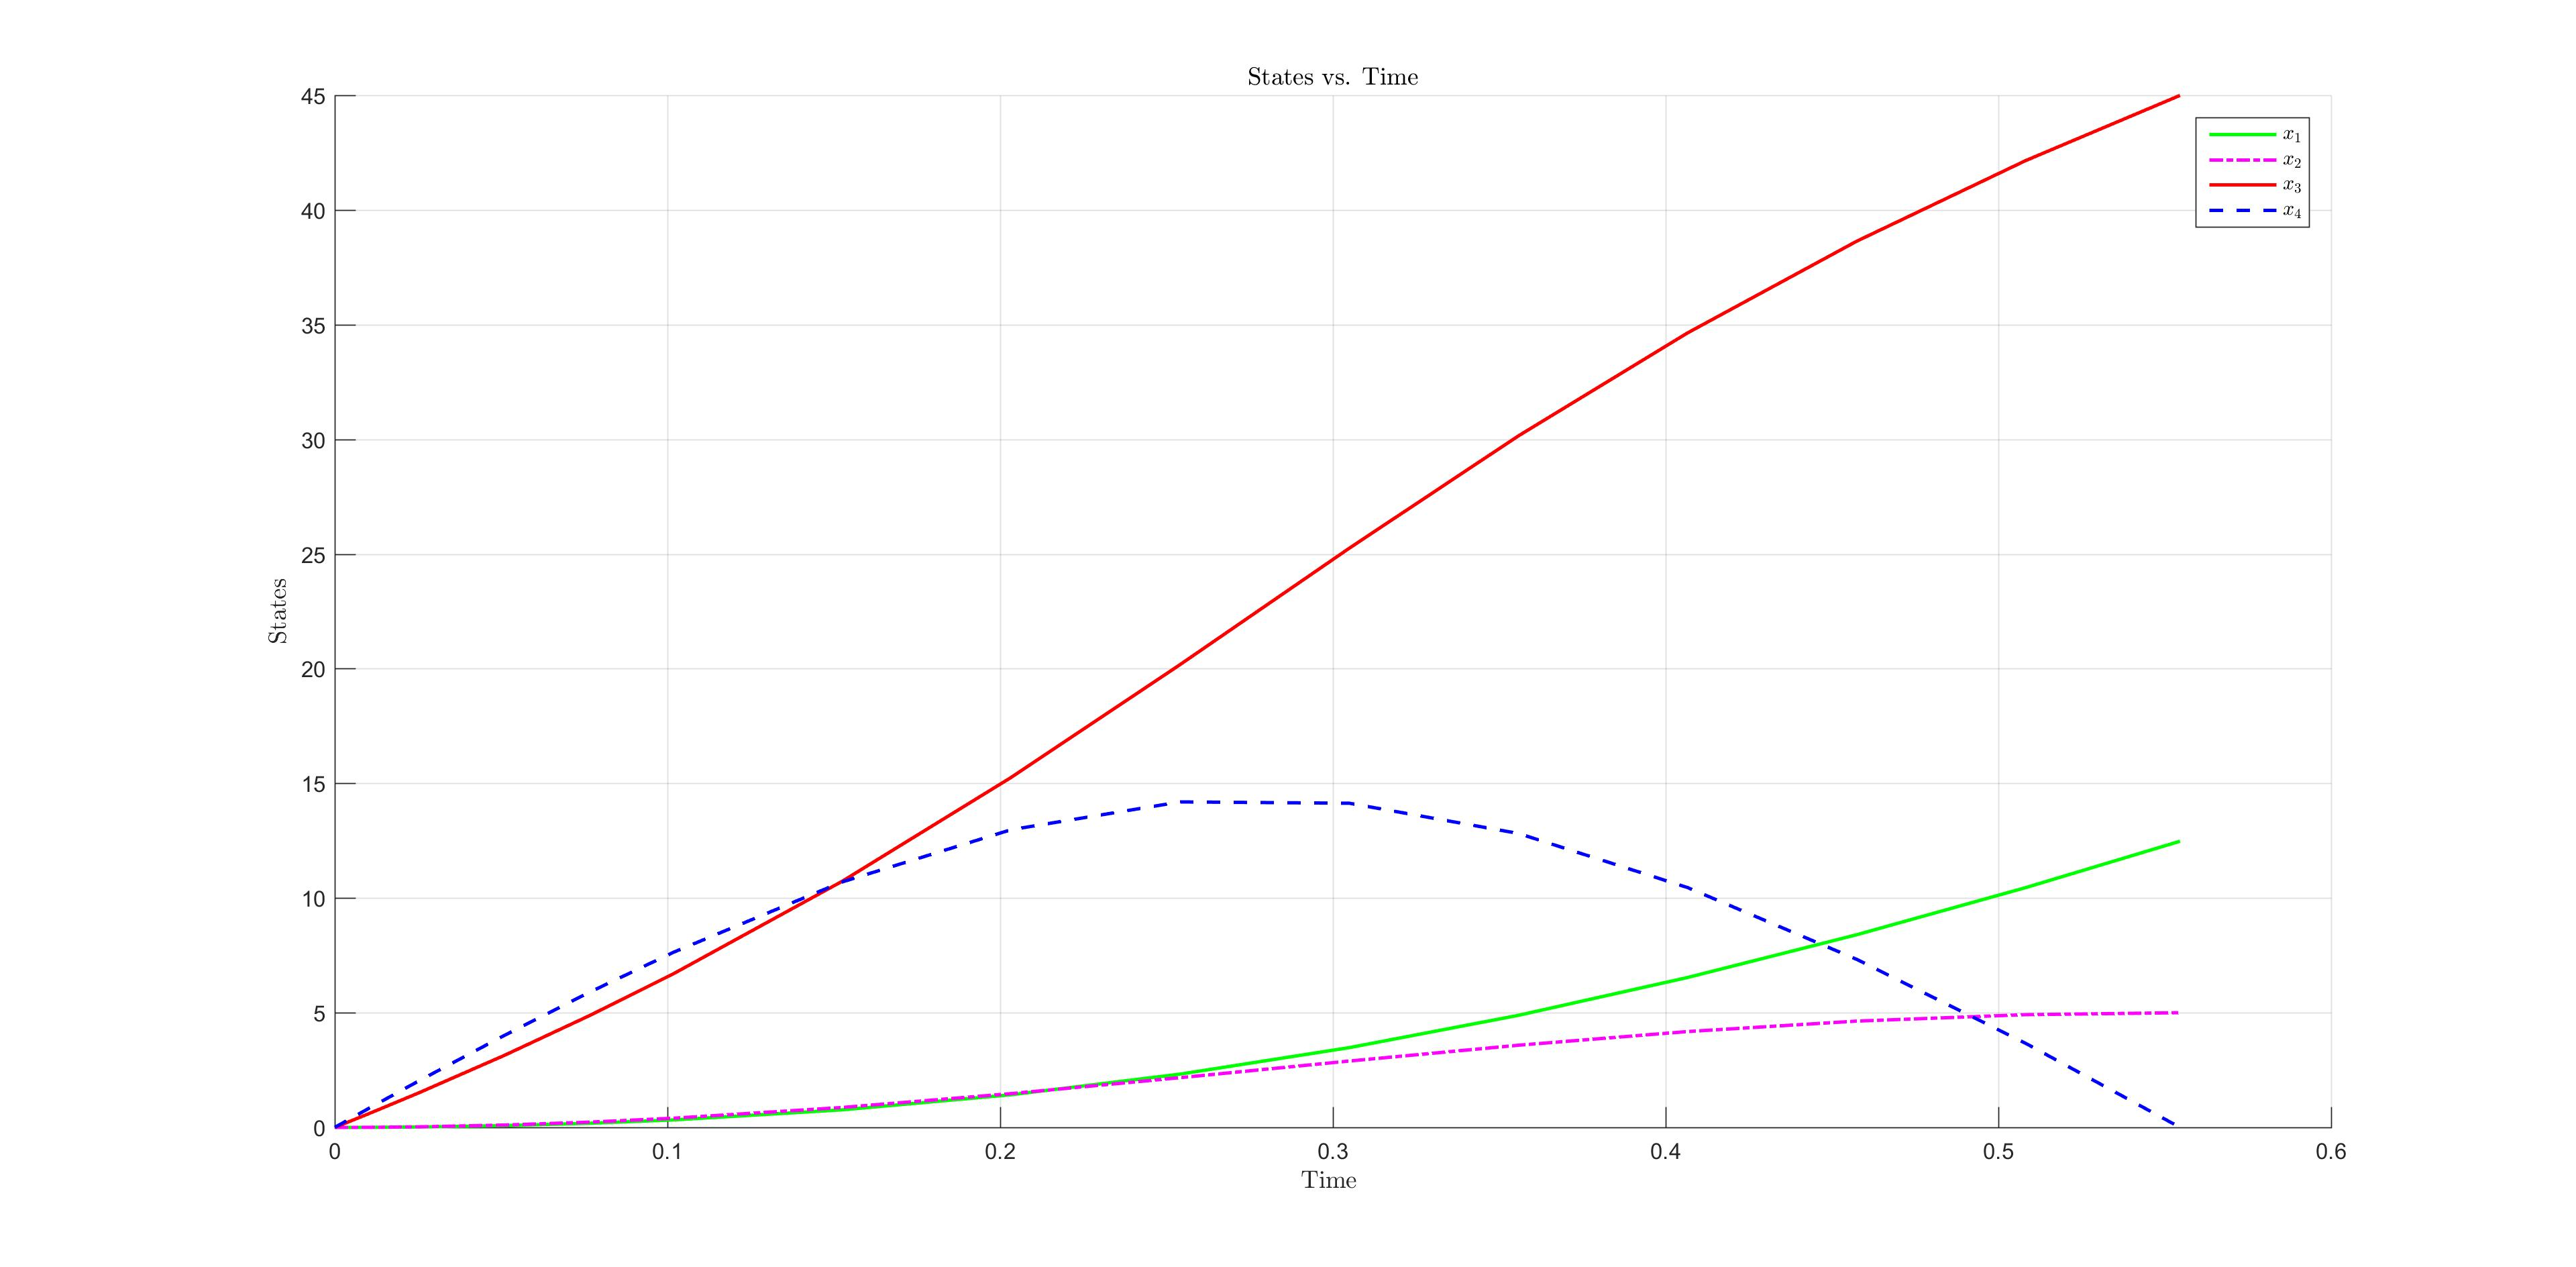
\includegraphics[scale=0.13]{HBVP_LTS_States.jpg}
		\caption{Linear Tangent Steering - HBVP - States}
	\end{figure}
	
	\begin{figure}[htpb]
		\centering
		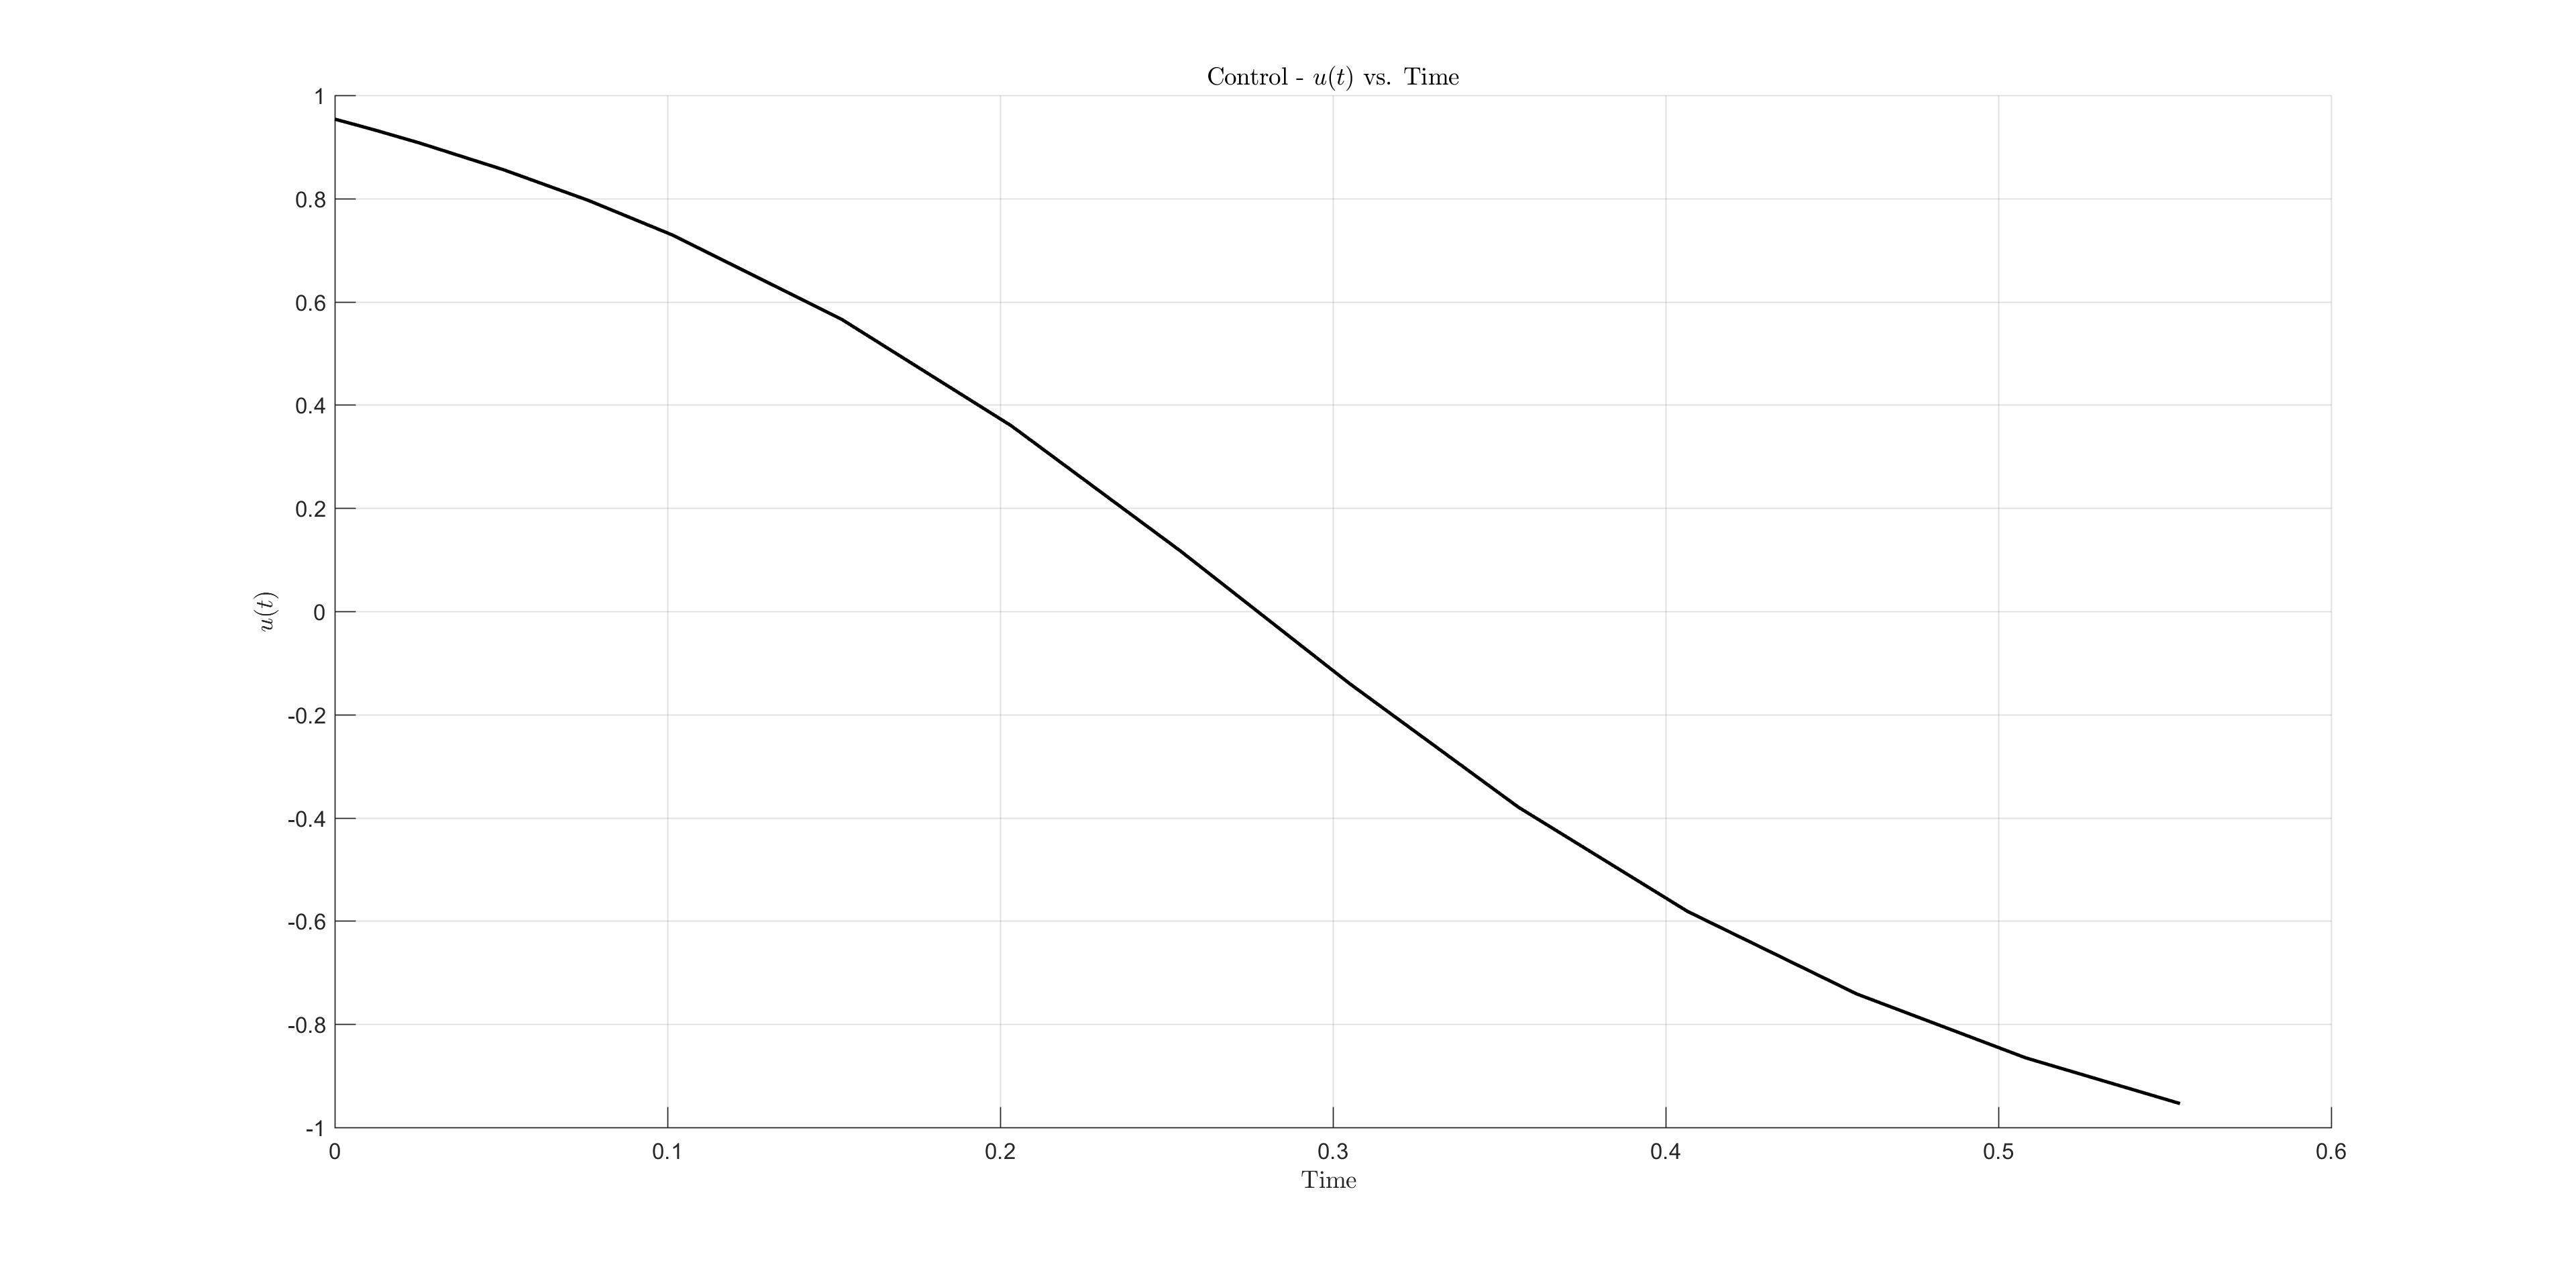
\includegraphics[scale=0.13]{HBVP_LTS_Control.jpg}
		\caption{Linear Tangent Steering - HBVP - Control}
	\end{figure}
	
	\begin{figure}[htpb]
		\centering
		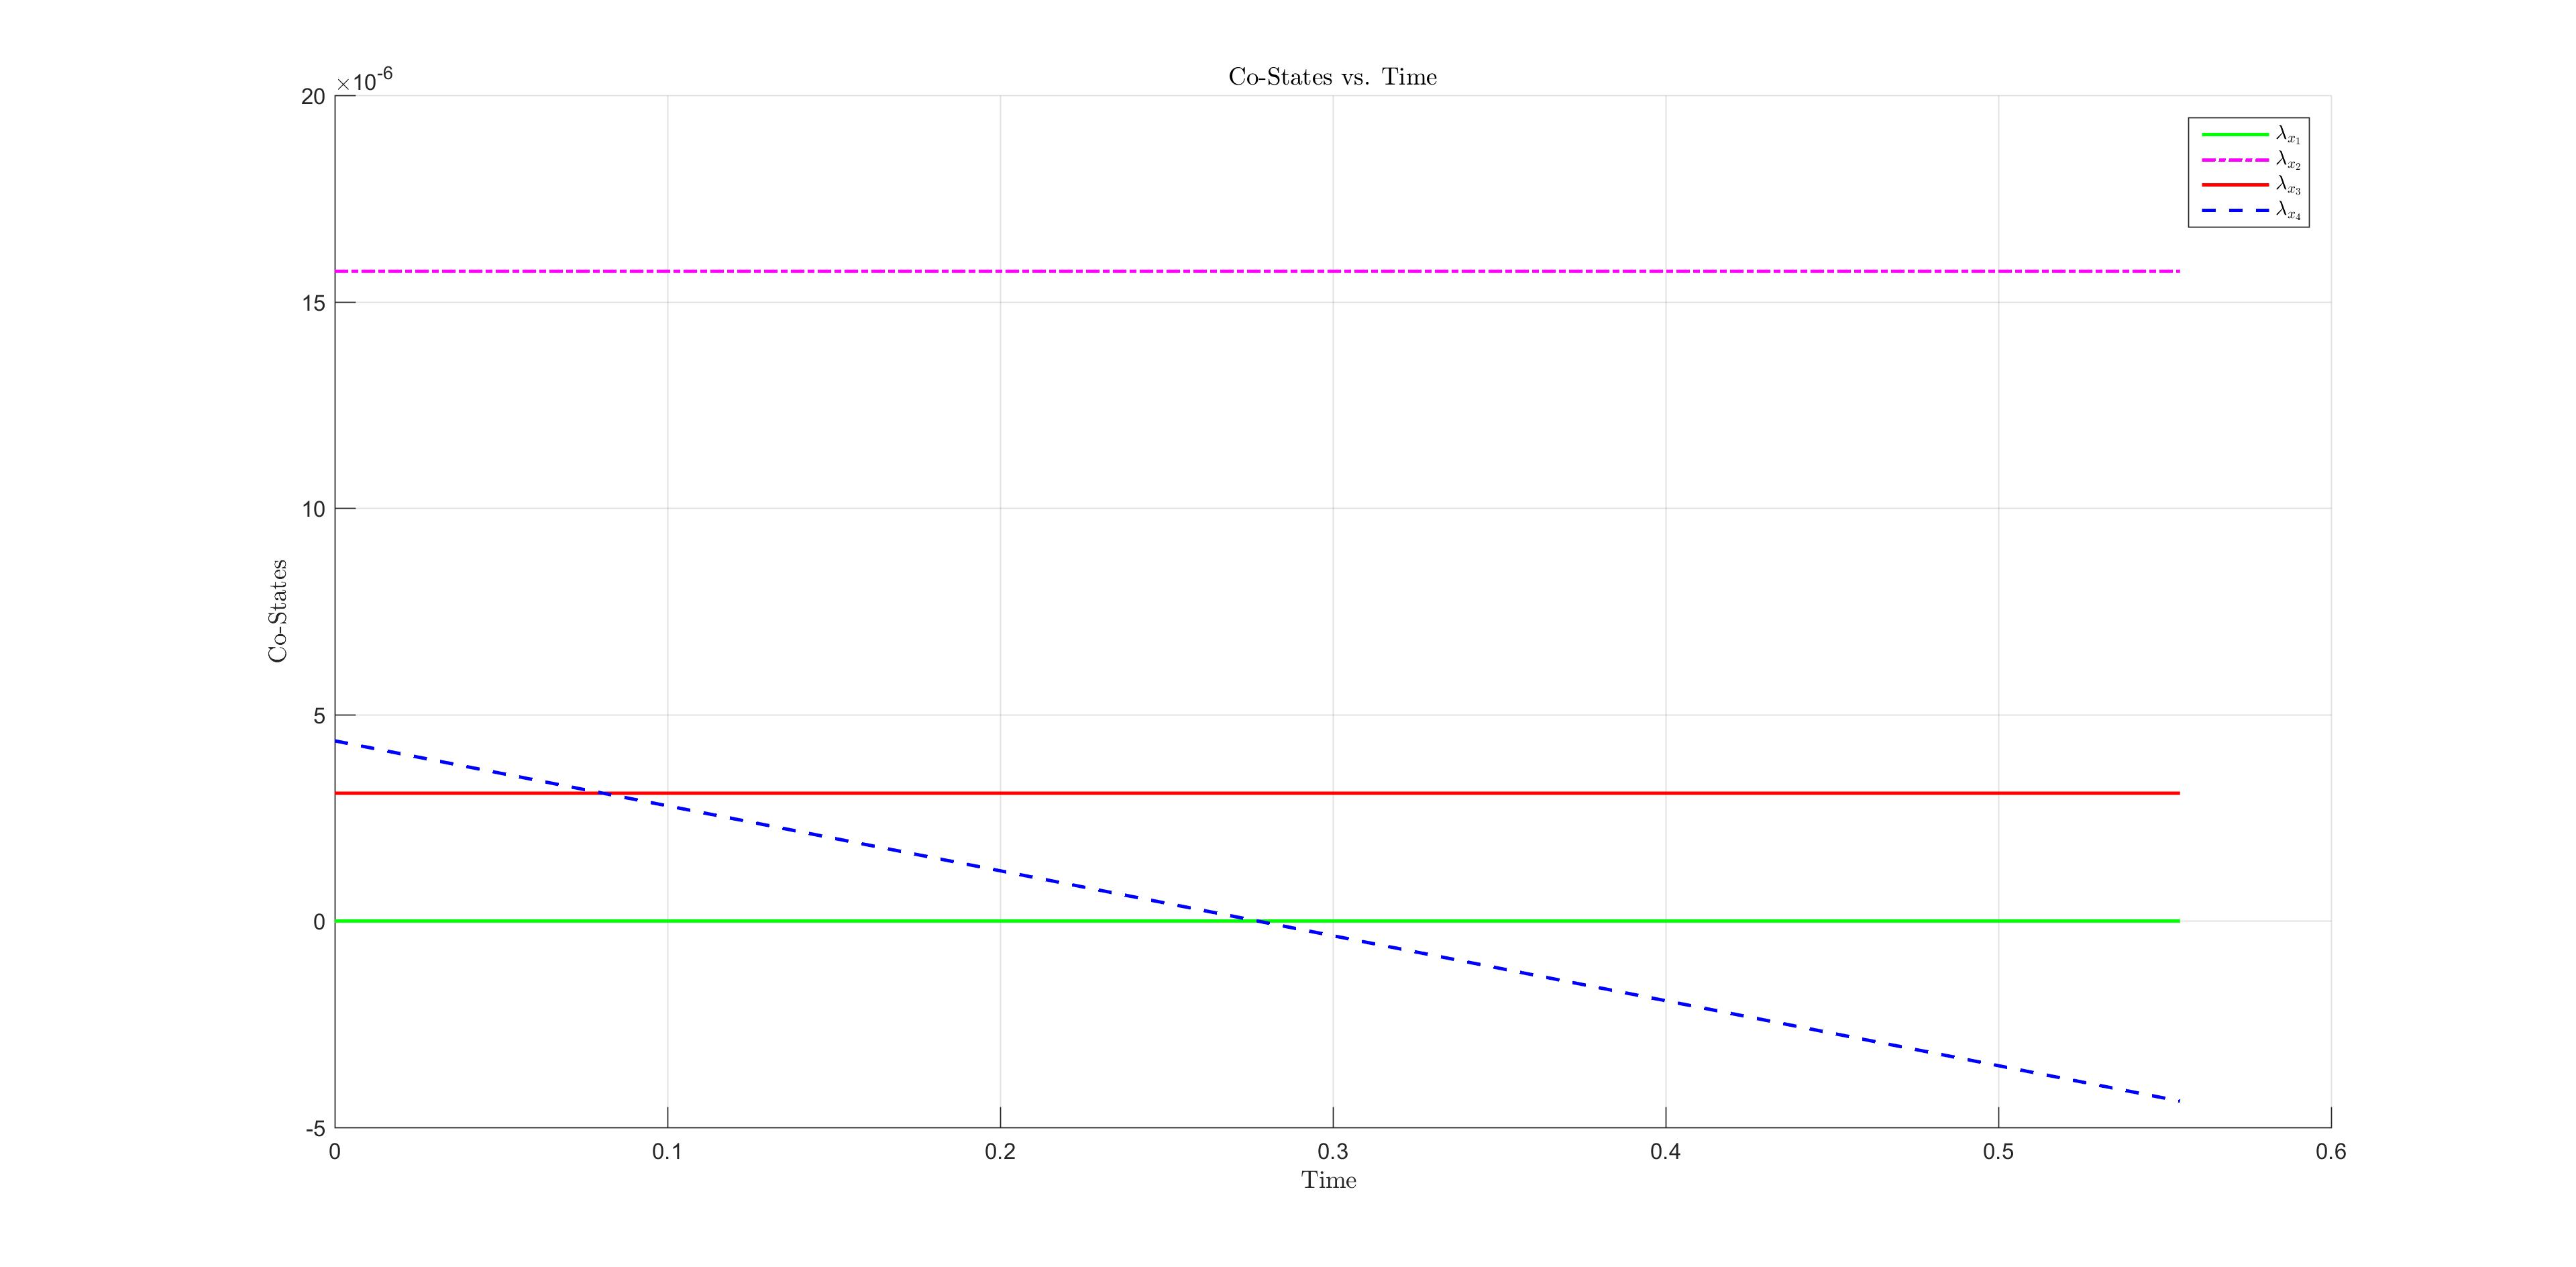
\includegraphics[scale=0.13]{HBVP_LTS_CoStates.jpg}
		\caption{Linear Tangent Steering - HBVP - CoStates}
	\end{figure}
	
	\newpage
	
	
	
	\subsection{Direct Method: Collocation}
	
	\subsubsection{Formulation of the NLP}
	
	The general Nonlinear Program (NLP) is given as follows,
	
	Minimize the cost functional,
	
	\begin{align} 
	J = F(\underbar Z),
	\end{align}
	
	Subject to the dynamic and path constraints constraints,
	
	\begin{align}
	\underbar g_{min} \leq \underbar g(\underbar Z) \leq \underbar g_{max},
	\end{align}
	
	With the following state constraints,
	
	\begin{align}
	\underbar Z_{min} \leq \underbar  Z \leq \underbar Z_{max},
	\end{align}
	
	For the Linear Tangent Steering Problem we have,
	
	\begin{align}
	\underbar Z &= 
	\begin{bmatrix}
	\underbar X_{1} \\ \underbar X_{2} \\ \underbar X_{3} \\ \underbar X_{4} \\ \underbar U \\ t_{0} \\ t_{f}
	\end{bmatrix}
	\end{align}
	
	Where,
	
	\begin{align}
	\underbar X_{1} &=
	\begin{bmatrix}
	x_{1}(1) \\ \vdots \\  x_{1}(N+1) 
	\end{bmatrix}
	& \underbar X_{2} &=
	\begin{bmatrix}
	x_{2}(1) \\  \vdots \\  x_{2}(N+1) 
	\end{bmatrix}
	& \underbar X_{3} &= 
	\begin{bmatrix}
	x_{3}(1) \\  \vdots \\  x_{3}(N+1) 
	\end{bmatrix}
	& \underbar X_{4} &= 
	\begin{bmatrix}
	x_{4}(1) \\  \vdots \\  x_{4}(N+1) 
	\end{bmatrix}
	& \underbar U &= 
	\begin{bmatrix}
	u(1) \\  \vdots \\  u(N) 
	\end{bmatrix} 
	\end{align}
	
	Where $N$ is the number of Legendre-Gauss-Radau (LGR) Points.
	
	Now we have $g( \underbar Z )$ as follows,
	
	\begin{align}
	g( \underbar Z ) &= 
	\begin{bmatrix}
	\bigtriangleup \underbar X_{1} \\  \bigtriangleup \underbar X_{2} \\ \bigtriangleup \underbar X_{3} \\  \bigtriangleup \underbar X_{4}
	\end{bmatrix}
	\end{align}
	
	The $\bigtriangleup \underbar X_{1}$, $\bigtriangleup \underbar X_{2}$, $\bigtriangleup \underbar X_{3}$ and $\bigtriangleup \underbar X_{4}$ are defined as follows,
	
	\begin{align}
	\bigtriangleup \underbar X_{1} &= D \underbar X_{1_{1:N+1} } - \frac{t_{f}}{2} \left[ x_{3_{1:N+1}} \right] &= \underbar 0, \nonumber \\
	\bigtriangleup \underbar X_{2} &= D \underbar X_{2_{1:N+1}} - \frac{t_{f}}{2} \left[ x_{4_{1:N+1}} \right]  &= \underbar 0,  \\
	\bigtriangleup \underbar X_{3} &= D \underbar X_{3_{1:N+1}} - \frac{t_{f}}{2} \left[ a.cos(u_{1:N}) \right]   &= \underbar 0, \nonumber \\
	\bigtriangleup \underbar X_{4} &= D \underbar X_{4_{1:N+1}} - \frac{t_{f}}{2} \left[ a.sin(u_{1:N}) \right]  &= \underbar 0, \nonumber 
	\end{align}
	
	Where $D$ is a differentiation matrix.\\
	
	The $ \underbar g_{min}$ and $ \underbar g_{max} $ are constant vectors of zeros since all the equations in (38) are equality constraints with zeros on the LHS, \\
	
	The $ \underbar Z_{min}$ and $ \underbar Z_{max} $ are constant vectors too but include the known boundary conditions and approximately correct lower and upper bounds for the decision vector contained in (35) as follows;
	
	\begin{align}
	\underbar Z_{min} &= 
	\begin{bmatrix}
	x_{1_{min}}(t_{0}) \\ x_{1_{min}}(t_{1}) \\  \vdots \\  x_{1_{min}}(t_{f}) \\  
	x_{2_{min}}(t_{0}) \\ x_{2_{min}}(t_{1}) \\ \vdots \\  x_{2_{min}}(t_{f}) \\ 
	x_{3_{min}}(t_{0}) \\ x_{3_{min}}(t_{1}) \\ \vdots \\  x_{3_{min}}(t_{f}) \\ 
	x_{4_{min}}(t_{0}) \\ x_{4_{min}}(t_{1}) \\ \vdots \\  x_{4_{min}}(t_{f}) \\ 
	u_{min}(t_{0}) \\ u_{min}(t_{1}) \\ \vdots \\  u_{min}(t_{f}) \\ 
	t_{0_{min}} \\ 
	t_{f_{min}}  
	\end{bmatrix}
	&=
	\begin{bmatrix}
	x_{1}(t_{0}) \\ x_{1_{min}}(t_{1}) \\ \vdots \\  x_{1_{min}}(t_{f}) \\  
	x_{2}(t_{0}) \\ x_{2_{min}}(t_{1}) \\ \vdots \\  x_{2}(t_{f}) \\ 
	x_{3}(t_{0}) \\ x_{3_{min}}(t_{1}) \\ \vdots \\  x_{3}(t_{f}) \\ 
	x_{4}(t_{0}) \\ x_{4_{min}}(t_{1}) \\ \vdots \\  x_{4}(t_{f}) \\ 
	u_{min}(t_{0}) \\ u_{min}(t_{1}) \\ \vdots \\  u_{min}(t_{f}) \\ 
	t_{0} \\ 
	t_{f_{min}}  
	\end{bmatrix}
	&=
	\begin{bmatrix}
	0 \\ 0 \\ \vdots \\  0 \\  
	0 \\ 0 \\ \vdots \\  5 \\ 
	0 \\ 0 \\ \vdots \\  45 \\ 
	0 \\ 0 \\ \vdots \\  0 \\ 
	-\pi /2 \\ -\pi /2 \\ \vdots \\  -\pi /2 \\ 
	0 \\ 
	0  
	\end{bmatrix}
	\end{align}
	
	\begin{align}
	\underbar Z_{max} &= 
	\begin{bmatrix}
	x_{1_{max}}(t_{0}) \\ x_{1_{max}}(t_{1}) \\ \vdots \\  x_{1_{max}}(t_{f}) \\  
	x_{2_{max}}(t_{0}) \\ x_{2_{max}}(t_{1}) \\ \vdots \\  x_{2_{max}}(t_{f}) \\ 
	x_{3_{max}}(t_{0}) \\ x_{3_{max}}(t_{1}) \\ \vdots \\  x_{3_{max}}(t_{f}) \\ 
	x_{4_{max}}(t_{0}) \\ x_{4_{max}}(t_{1}) \\ \vdots \\  x_{4_{max}}(t_{f}) \\ 
	u_{max}(t_{0}) \\ u_{max}(t_{1}) \\ \vdots \\  u_{max}(t_{f}) \\ 
	t_{0_{max}} \\ 
	t_{f_{max}}  
	\end{bmatrix}
	&=
	\begin{bmatrix}
	x_{1_{max}}(t_{0}) \\ x_{1_{max}}(t_{1}) \\ \vdots \\  x_{1_{max}}(t_{f}) \\  
	x_{2}(t_{0}) \\ x_{2_{max}}(t_{1}) \\ \vdots \\  x_{2}(t_{f}) \\ 
	x_{3}(t_{0}) \\ x_{3_{max}}(t_{1}) \\ \vdots \\  x_{3}(t_{f}) \\ 
	x_{4}(t_{0}) \\ x_{4_{max}}(t_{1}) \\ \vdots \\  x_{4}(t_{f}) \\ 
	u_{max}(t_{0}) \\ u_{max}(t_{1}) \\ \vdots \\  u_{max}(t_{f}) \\ 
	t_{0} \\ 
	t_{f_{max}}  
	\end{bmatrix}
	&=
	\begin{bmatrix}
	100 \\ 100 \\ \vdots \\  100 \\  
	0 \\ 100 \\ \vdots \\  5 \\ 
	0 \\ 100 \\ \vdots \\  45 \\ 
	0 \\ 100 \\ \vdots \\  0 \\ 
	\pi /2 \\ \pi /2 \\ \vdots \\  \pi /2 \\ 
	0 \\ 
	100  
	\end{bmatrix}
	\end{align}
	
	Note: In equations (39) and (40) the vertical dots in the numerical vector represent values that are equal to the value before the dots begin.
	
	Now the problem defined by the equations (32), (33) and (34) is solved using a NLP solver which in this case is IPOPT. Moreover, this NLP solver has two modes as follows, 
	
	\begin{itemize}
		\item Full Newton: We have to provide Objective Function Gradient, Constraint Jacobian and Hessian of the NLP Lagrangian to the solver.
		\item Quasi-Newton: We have to provide Objective Function Gradient and Constraint Jacobian to the solver.
	\end{itemize}
	
	In our case, we solve our NLP in IPOPT using the Quasi-Newton mode and hence, provide the IPOPT solver with Objective Function Gradient and Constraint Jacobian computed by ADiGator (Algorithmic Differentiator) as follows, \\
	
	The Objective Function Gradient is given as,
	
	\begin{align}
	\frac{\partial F}{\partial \underbar Z} &= \left[ \quad \frac{\partial F}{\partial \underbar X_{1}} \quad \frac{\partial F}{\partial \underbar X_{2}} \quad \frac{\partial F}{\partial \underbar X_{3}} \quad \frac{\partial F}{\partial \underbar X_{4}} \quad \frac{\partial F}{\partial \underbar U} \quad \frac{\partial F}{\partial t_{0}} \quad \frac{\partial F}{\partial t_{f}} \right]
	\end{align}
	
	The Constraint Jacobian is given as,
	
	\begin{align}
	\frac{\partial \underbar g}{\partial \underbar Z}  &= \left[ \quad \frac{\partial \underbar g}{\partial \underbar X_{1}} \quad \frac{\partial \underbar g}{\partial \underbar X_{2}} \quad \frac{\partial \underbar g}{\partial \underbar X_{3}} \quad \frac{\partial \underbar g}{\partial \underbar X_{4}} \quad \frac{\partial \underbar g}{\partial \underbar U} \quad \frac{\partial \underbar g}{\partial t_{0}} \quad \frac{\partial \underbar g}{\partial t_{f}} \right]
	\end{align}
	
	Note: Each element in the LHS of equation (41) is a row vector, hence the LHs is a large row vector; and each element in the LHS of equation (42) is a column vector, hence the LHS is a large matrix.
	
	
	\newpage
	
	
	\subsubsection{MATLAB Code}
	
	\lstinputlisting{LinearTangentMain.m}
	
	\newpage
	
	\lstinputlisting{LinearTangentObj.m}
	
	\newpage
	
	\lstinputlisting{LinearTangentFun.m}
	
	\newpage
	
	\lstinputlisting{LinearTangentCon.m}
	
	\lstinputlisting{LinearTangentGrd.m}
	
	\lstinputlisting{LinearTangentJac.m}
	
	\lstinputlisting{LinearTangentJacPat.m}
	
	\newpage
	
	
	\subsubsection{Results}
	
	\begin{figure}[htpb]
		\centering
		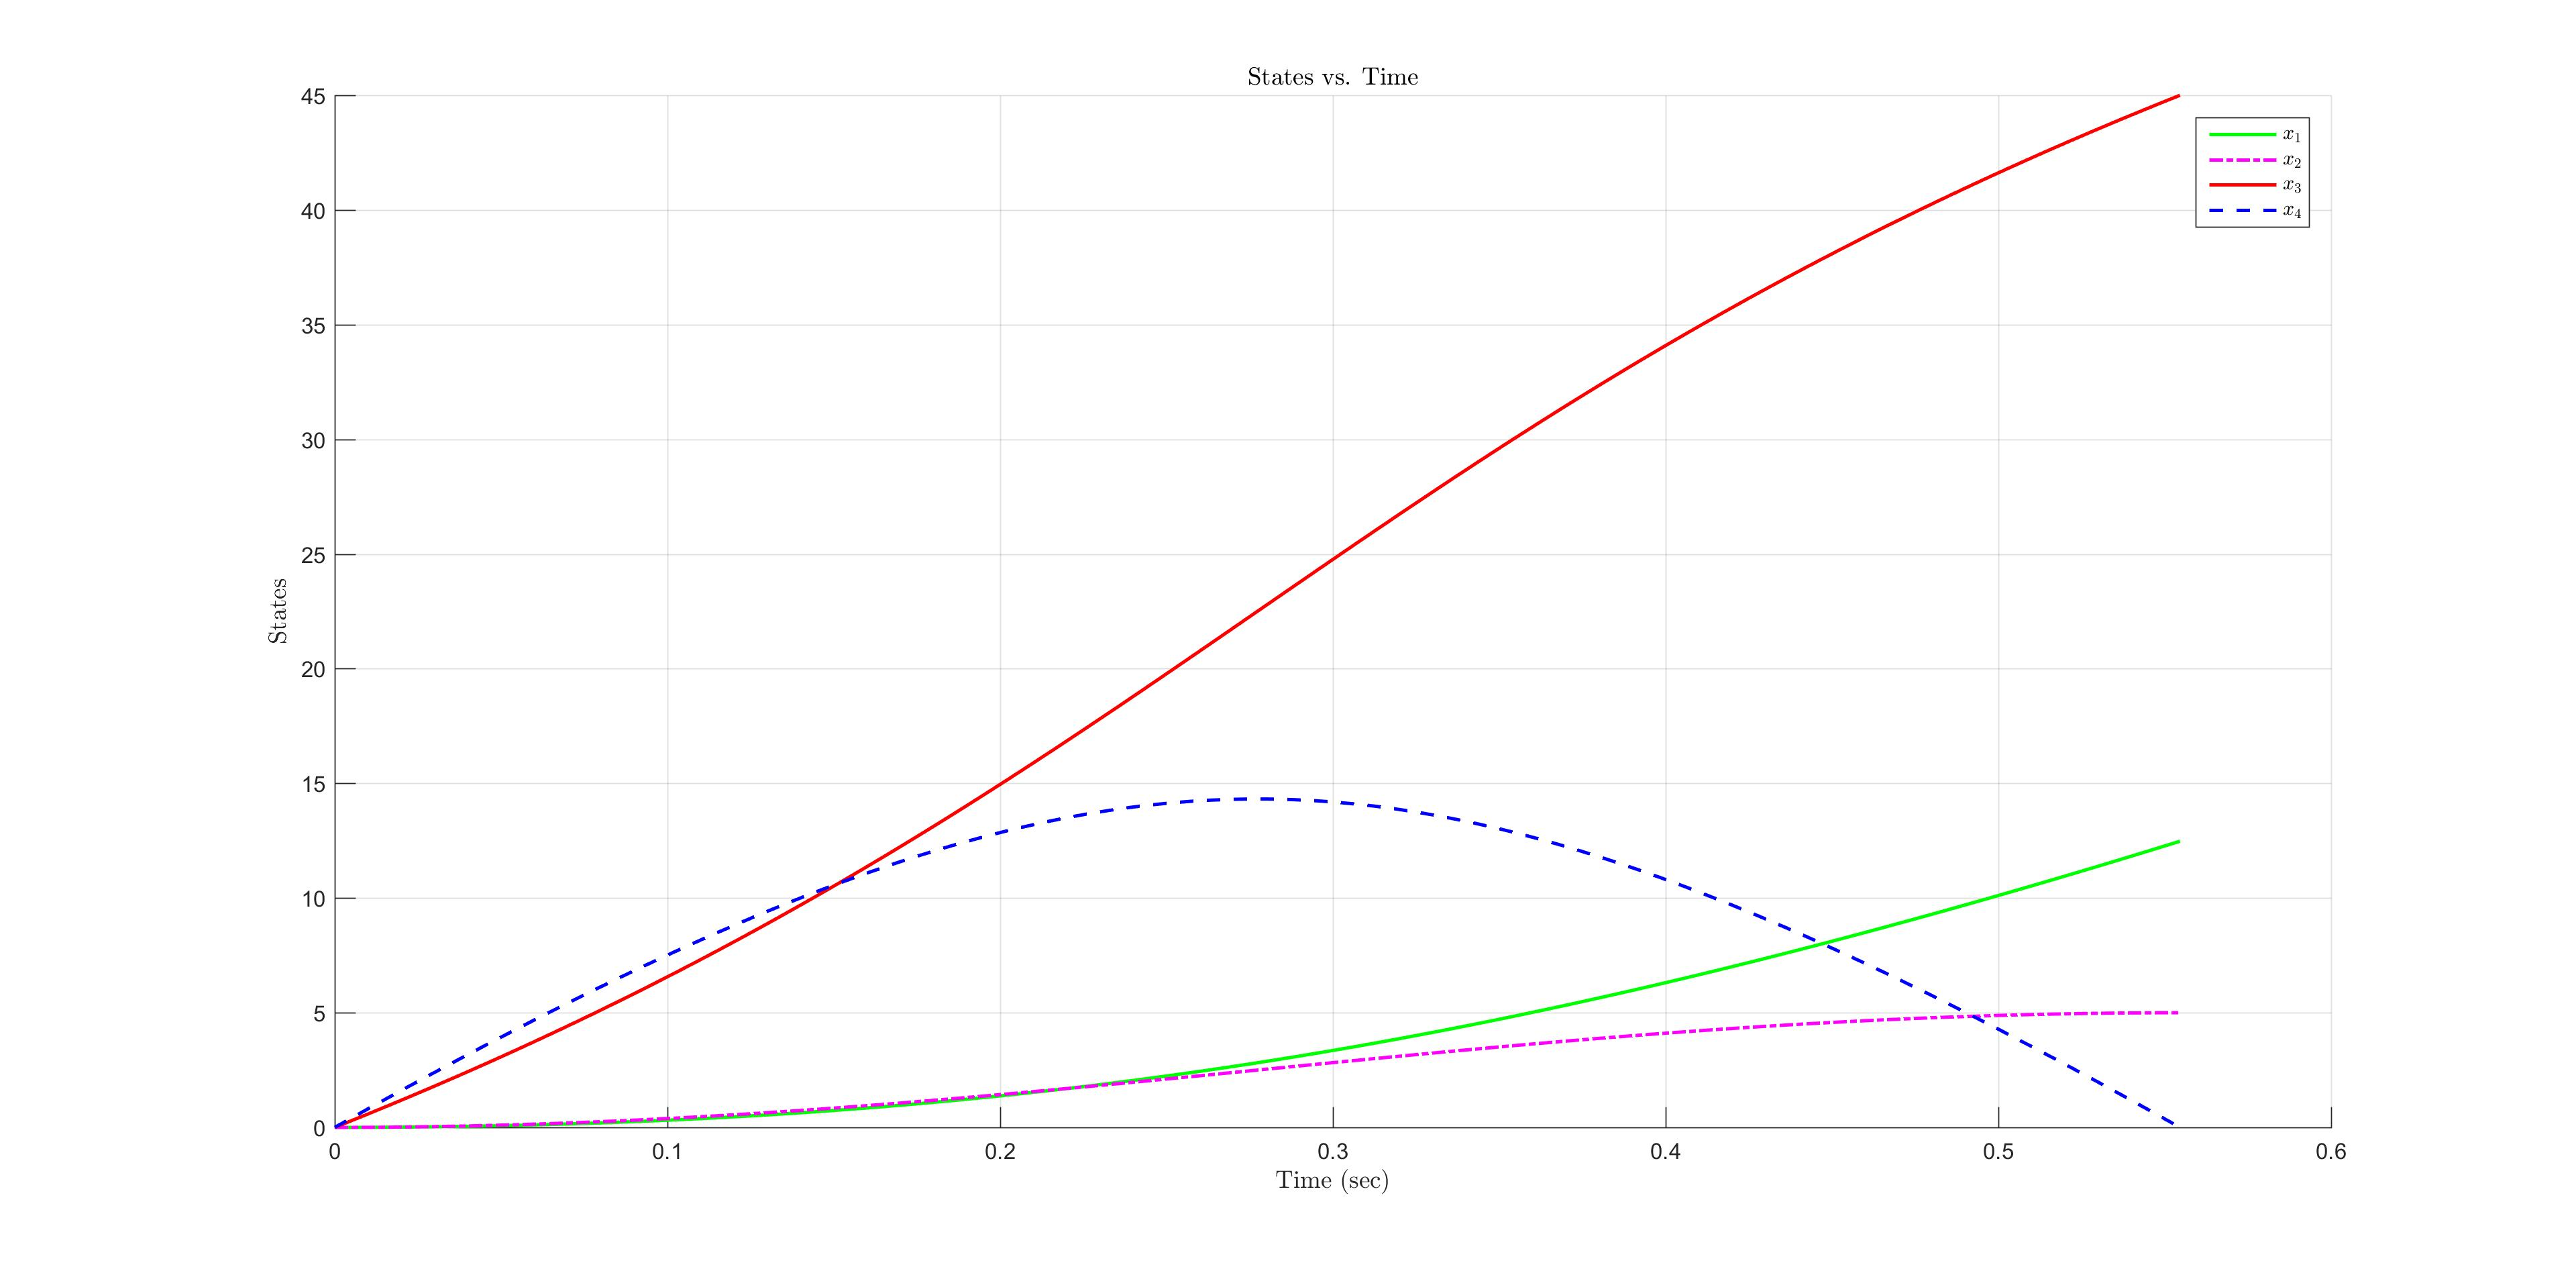
\includegraphics[scale=0.13]{Collocation_LTS_States.jpg}
		\caption{Linear Tangent Steering - Collocation - States}
	\end{figure}
	
	\begin{figure}[htpb]
		\centering
		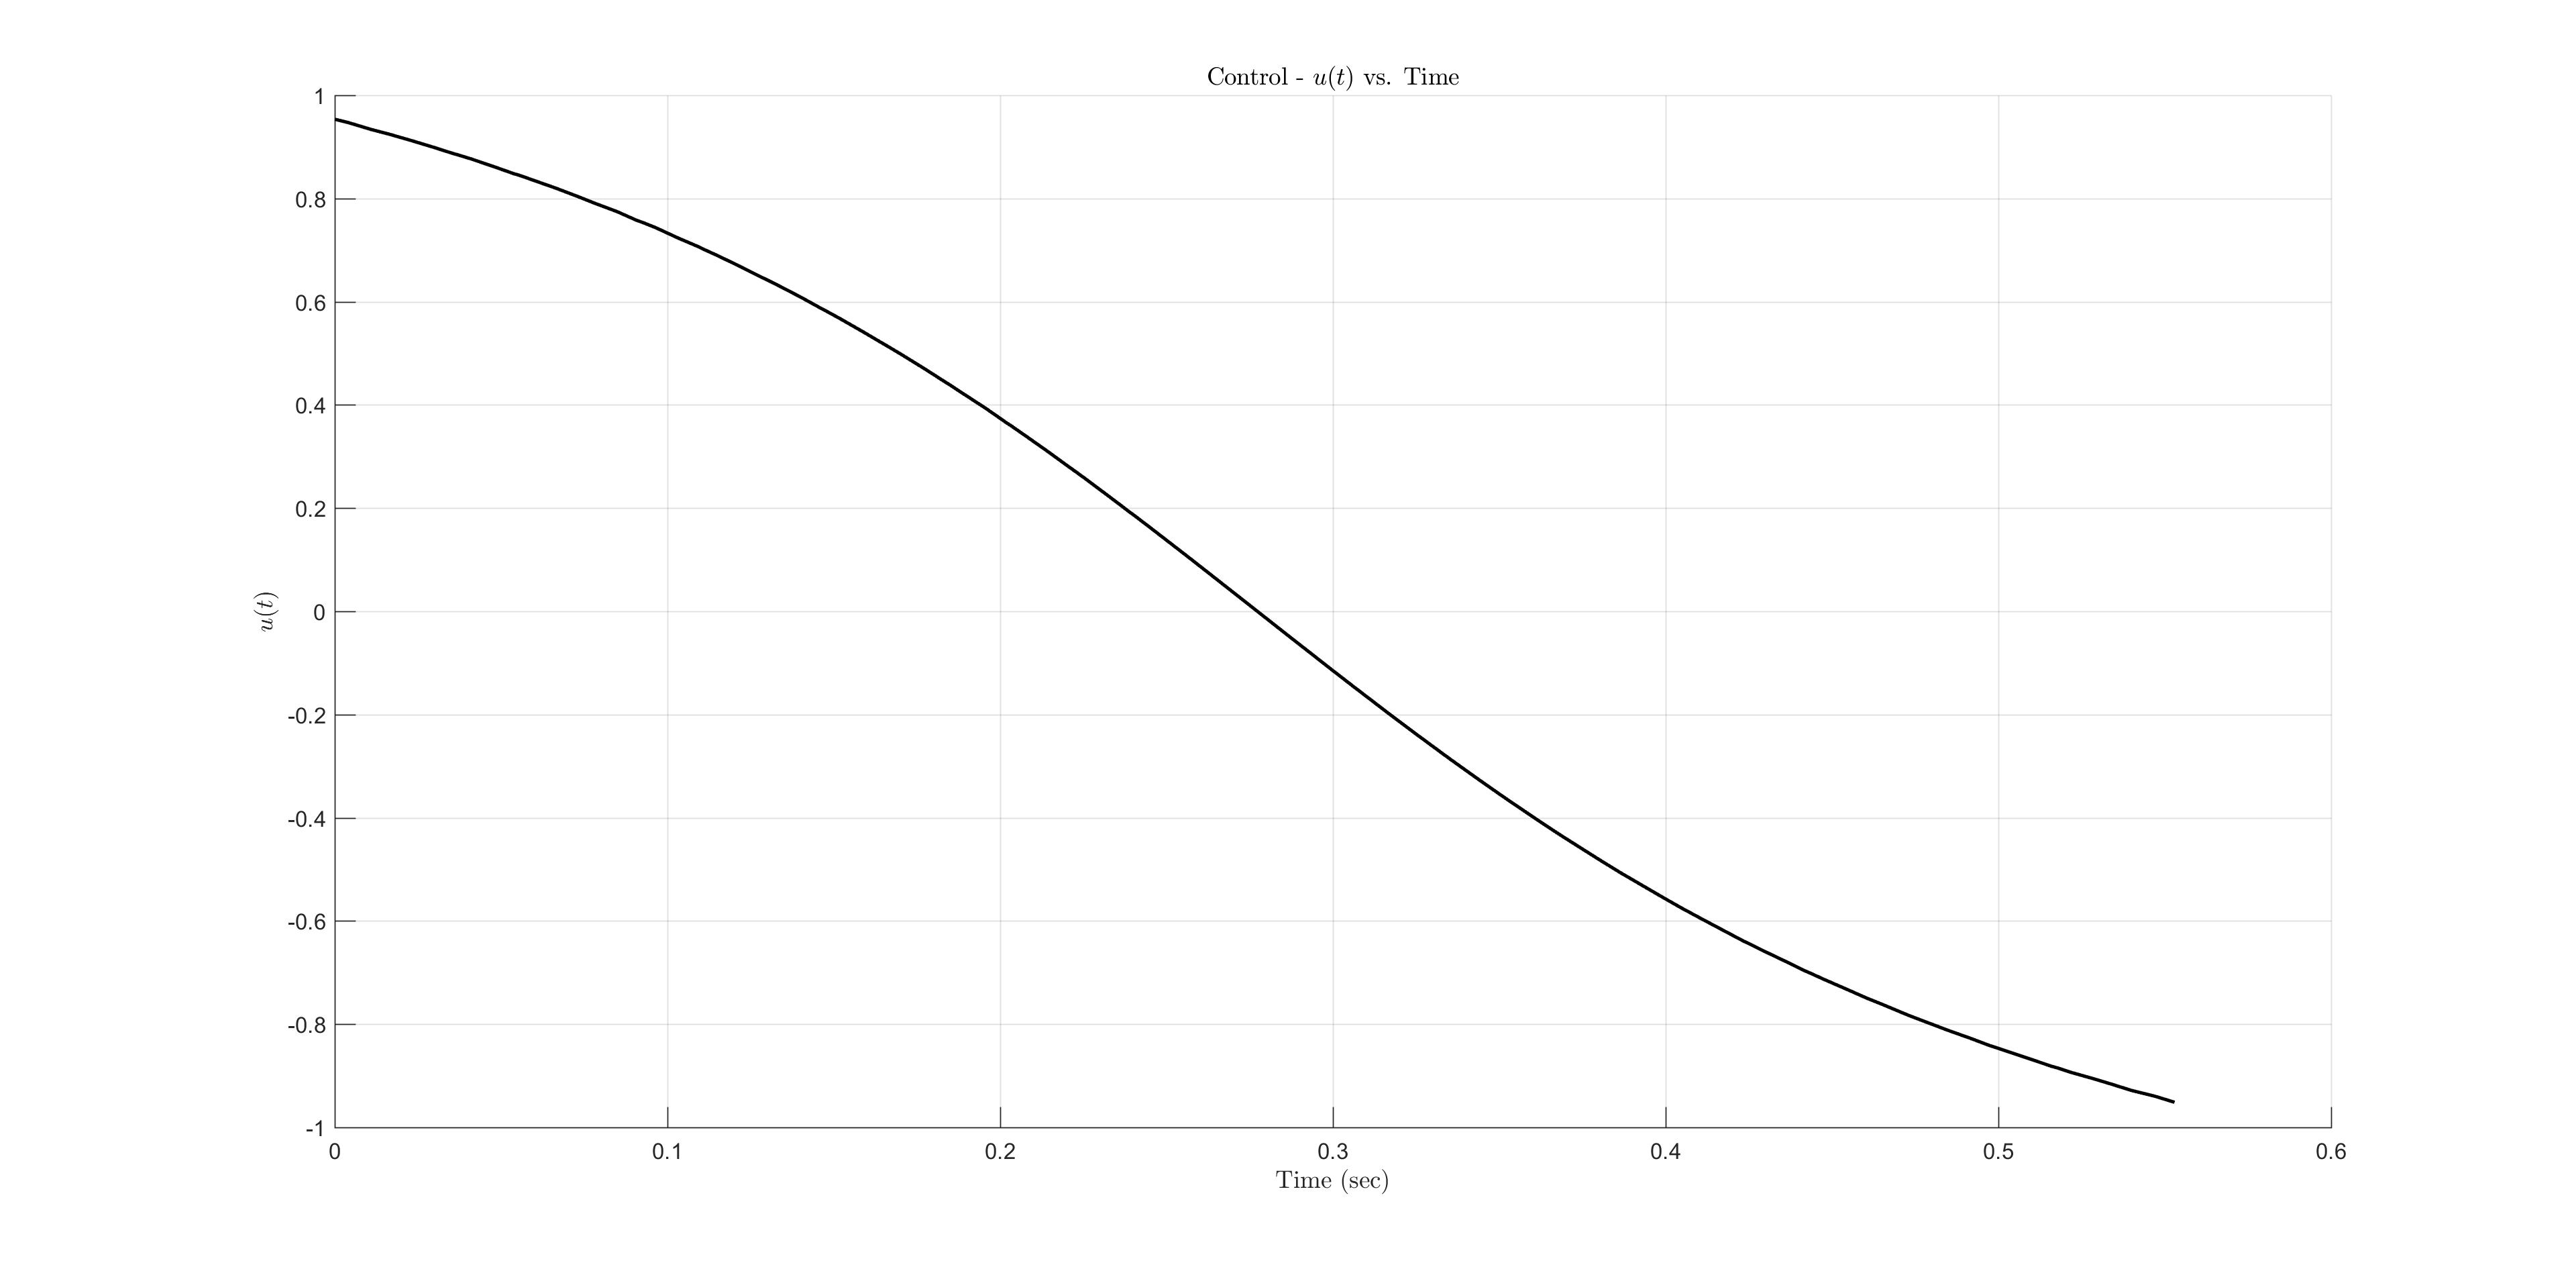
\includegraphics[scale=0.13]{Collocation_LTS_Control.jpg}
		\caption{Linear Tangent Steering - Collocation - Control}
	\end{figure}
	
	\begin{figure}[htpb]
		\centering
		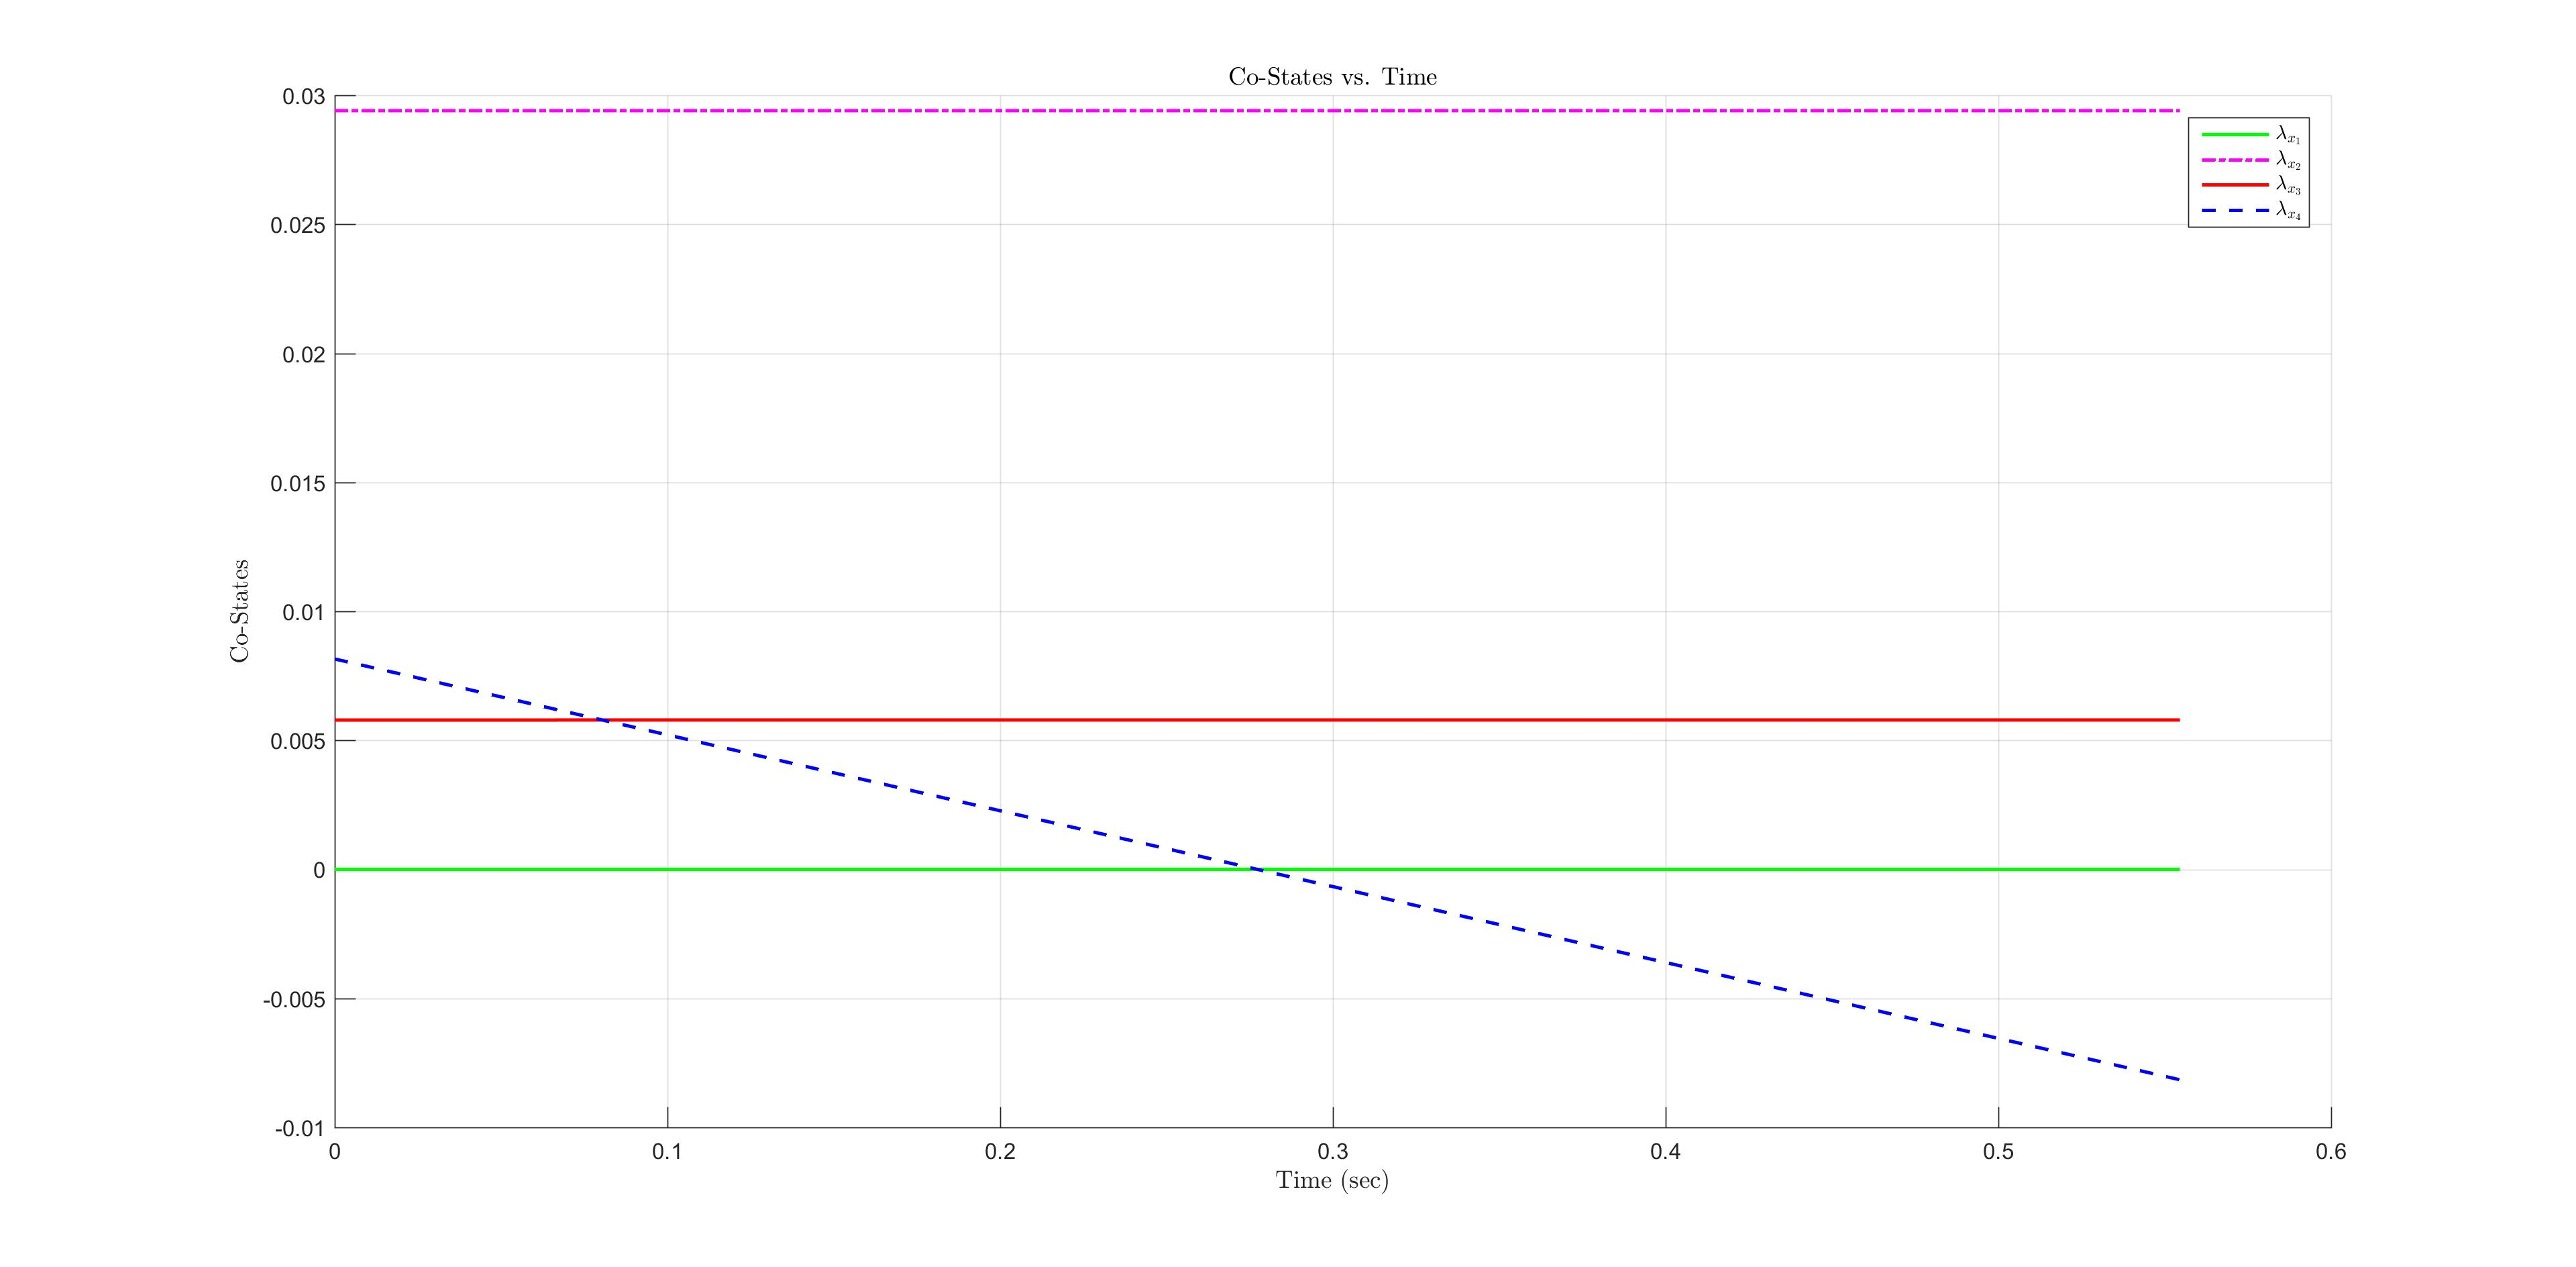
\includegraphics[scale=0.13]{Collocation_LTS_CoStates.jpg}
		\caption{Linear Tangent Steering - Collocation - CoStates}
	\end{figure}
	
	\newpage
	
	
	
	\subsection{Analysis}
	
	\subsubsection{Quality of Numerical Approximations}
	
	\begin{enumerate}
		\item For the Linear Tangent Steering problem the solutions from both the HBVP and Collocation methods are equivalent. 
		\item Even when initial conditions for both the HBVP and Collocation methods are changed the optimal solution remains the same; hence, showing the robustness of both the methods.
	\end{enumerate}
	
	\subsubsection{Key Computational Issues}
	
	\begin{enumerate}
		\item The time taken to solve by the HBVP (1.2847 sec) is approximately three times the time taken by the Collocation method (0.4771 sec). Hence, Collocation method is computationally faster.
		\item The Collocation method ends with the solver exiting with status of "Optimal solution found"; however the root finder in the HBVP method exits with the status "last step was ineffective", but when the TolFun tolerance is relaxed it is able to solve the equation .
		\item Overall setting up the Collocation problem is easier as compared to HBVP; as one does not have to analytically solve for the first order optimality conditions. However, tools like ADiGator which compute the Gradient, Jacobian and Hessian of the Objective, Constraints and NLP Lagrangian respectively actually make the process of setting up the Collocation problem.
	\end{enumerate}
	
	\newpage
	
	
	\section{Advanced Problem: Robot Arm}
	
	
	\subsection{Problem Formulation:}
	
	The Robot Arm Optimal Control Problem is as follows;\\
	
	Minimize the cost functional,
	
	\begin{align} 
	J = t_{f},
	\end{align}
	
	Subject to the dynamic constraints,
	
	\begin{align}
	\dot x_{1} &= x_{2}, \nonumber\\
	\dot x_{2} &= u_{1}/L, \nonumber\\
	\dot x_{3} &= x_{4},\\
	\dot x_{4} &= u_{2}/I_{\theta}, \nonumber\\
	\dot x_{5} &= x_{6,} \nonumber\\
	\dot x_{6} &= u_{3}/I_{\phi}, \nonumber
	\end{align}
	
	With the control inequalities,,
	
	\begin{align} 
	|u_{i}| \leq 1 \quad , \quad (i=1,2,3),
	\end{align}
	
	With the following boundary conditions,
	
	\begin{align}
	t_{0} &= 0 & t_{f} &= \text{Free}, \nonumber \\
	x_{1}(0) &= 4.5 & x_{1}(t_{f}) &= 4.5, \nonumber \\
	x_{2}(0) &= 0 & x_{2}(t_{f}) &= 0,  \nonumber\\
	x_{3}(0) &= 0 & x_{3}(t_{f}) &= 2\pi/3, \\
	x_{3}(0) &= 0 & x_{3}(t_{f}) &= 0, \nonumber \\
	x_{4}(0) &= \pi/4 & x_{4}(t_{f}) &= \pi/4, \nonumber \\
	x_{5}(0) &= 0 & x_{5}(t_{f}) &= 0, \nonumber 
	\end{align}
	
	Where $L=5$ and $I_{\theta}$ and $I_{\phi}$ are as follows,
	
	\begin{align}
	I_{\theta} &= \frac{1}{3} \left[ \left(  L-x_{1}\right) ^{3} + x_{1}^{3}\right] ,\\
	I_{\phi} &= I_{\theta}sin^{2}(x_{5}), 
	\end{align}
	
	
	\newpage
	
	
	\subsection{Direct Method: Collocation}
	
	\subsubsection{Formulation of the NLP}
	
	The general Nonlinear Program (NLP) is given as follows,
	
	Minimize the cost functional,
	
	\begin{align} 
	J = F(\underbar Z),
	\end{align}
	
	Subject to the dynamic and path constraints constraints,
	
	\begin{align}
	\underbar g_{min} \leq \underbar g(\underbar Z) \leq \underbar g_{max},
	\end{align}
	
	With the following state constraints,
	
	\begin{align}
	\underbar Z_{min} \leq \underbar  Z \leq \underbar Z_{max},
	\end{align}
	
	For the Linear Tangent Steering Problem we have,
	
	\begin{align}
	\underbar Z &= 
	\begin{bmatrix}
	\underbar X_{1} \\ \underbar X_{2} \\ \underbar X_{3} \\ \underbar X_{4} \\ \underbar X_{5} \\ \underbar X_{6} \\ \underbar U_{1} \\ \underbar U_{2} \\ \underbar U_{3} \\ t_{0} \\ t_{f}
	\end{bmatrix}
	\end{align}
	
	Where,
	
	\begin{align}
	\underbar X_{1} &=
	\begin{bmatrix}
	x_{1}(1) \\ \vdots \\  x_{1}(N+1) 
	\end{bmatrix}
	& \underbar X_{2} &=
	\begin{bmatrix}
	x_{2}(1) \\  \vdots \\  x_{2}(N+1) 
	\end{bmatrix}
	& \underbar X_{3} &= 
	\begin{bmatrix}
	x_{3}(1) \\  \vdots \\  x_{3}(N+1) 
	\end{bmatrix}
	& \underbar X_{4} &= 
	\begin{bmatrix}
	x_{4}(1) \\  \vdots \\  x_{4}(N+1) 
	\end{bmatrix}
	& \underbar X_{5} &= 
	\begin{bmatrix}
	x_{5}(1) \\  \vdots \\  x_{5}(N+1)  
	\end{bmatrix} 
	\end{align}
	
	\begin{align}
	\underbar X_{6} &=
	\begin{bmatrix}
	x_{6}(1) \\ \vdots \\  x_{6}(N+1) 
	\end{bmatrix}
	& \underbar U_{1} &=
	\begin{bmatrix}
	u_{1}(1) \\  \vdots \\  u_{1}(N) 
	\end{bmatrix}
	& \underbar U_{2} &= 
	\begin{bmatrix}
	u_{2}(1) \\  \vdots \\  u_{2}(N) 
	\end{bmatrix}
	& \underbar U_{3} &= 
	\begin{bmatrix}
	u_{4}(1) \\  \vdots \\  u_{4}(N) 
	\end{bmatrix}
	\end{align}
	
	Where $N$ is the number of Legendre-Gauss-Radau (LGR) Points.
	
	Now we have $g( \underbar Z )$ as follows,
	
	\begin{align}
	g( \underbar Z ) &= 
	\begin{bmatrix}
	\bigtriangleup \underbar X_{1} \\  \bigtriangleup \underbar X_{2} \\ \bigtriangleup \underbar X_{3} \\  \bigtriangleup \underbar X_{4} \\  \bigtriangleup \underbar X_{5} \\  \bigtriangleup \underbar X_{6}
	\end{bmatrix}
	\end{align}
	
	The $\bigtriangleup \underbar X_{1}$, $\bigtriangleup \underbar X_{2}$, $\bigtriangleup \underbar X_{3}$, $\bigtriangleup \underbar X_{4}$, $\bigtriangleup \underbar X_{5}$ and $\bigtriangleup \underbar X_{6}$ are defined as follows,
	
	\begin{align}
	\bigtriangleup \underbar X_{1} &= D \underbar X_{1_{1:N+1} } - \frac{t_{f}}{2} \left[ x_{2_{1:N+1}} \right] &= \underbar 0, \nonumber \\
	\bigtriangleup \underbar X_{2} &= D \underbar X_{2_{1:N+1}} - \frac{t_{f}}{2} \left[ u_{1_{1:N}}/L \right]  &= \underbar 0, \nonumber \\
	\bigtriangleup \underbar X_{3} &= D \underbar X_{3_{1:N+1}} - \frac{t_{f}}{2} \left[ x_{4_{1:N+1}} \right]   &= \underbar 0,  \\
	\bigtriangleup \underbar X_{4} &= D \underbar X_{4_{1:N+1}} - \frac{t_{f}}{2} \left[ u_{2_{1:N}}/I_{\theta} \right]  &= \underbar 0, \nonumber \\ 
	\bigtriangleup \underbar X_{5} &= D \underbar X_{5_{1:N+1}} - \frac{t_{f}}{2} \left[ x_{6_{1:N+1}} \right]  &= \underbar 0, \nonumber \\
	\bigtriangleup \underbar X_{6} &= D \underbar X_{6_{1:N+1}} - \frac{t_{f}}{2} \left[ u_{3_{1:N}}/I_{\phi} \right]  &= \underbar 0, \nonumber 
	\end{align}
	
	Where $D$ is a differentiation matrix and $L$, $I_{\theta}$ and $I_{\phi}$ are as defined in the previous section.\\
	
	The $ \underbar g_{min}$ and $ \underbar g_{max} $ are constant vectors of zeros since all the equations in (56) are equality constraints with zeros on the LHS, \\
	
	The $ \underbar Z_{min}$ and $ \underbar Z_{max} $ are constant vectors too but include the known boundary conditions and approximately correct lower and upper bounds for the decision vector contained in (52) as follows;
	
	\begin{align}
	\underbar Z_{min} &= 
	\begin{bmatrix}
	x_{1_{min}}(t_{0}) \\ x_{1_{min}}(t_{1}) \\  \vdots \\  x_{1_{min}}(t_{f}) \\  
	x_{2_{min}}(t_{0}) \\ x_{2_{min}}(t_{1}) \\ \vdots \\  x_{2_{min}}(t_{f}) \\ 
	x_{3_{min}}(t_{0}) \\ x_{3_{min}}(t_{1}) \\ \vdots \\  x_{3_{min}}(t_{f}) \\ 
	x_{4_{min}}(t_{0}) \\ x_{4_{min}}(t_{1}) \\ \vdots \\  x_{4_{min}}(t_{f}) \\ 
	x_{5_{min}}(t_{0}) \\ x_{5_{min}}(t_{1}) \\ \vdots \\  x_{5_{min}}(t_{f}) \\
	x_{6_{min}}(t_{0}) \\ x_{6_{min}}(t_{1}) \\ \vdots \\  x_{6_{min}}(t_{f}) \\
	u_{1_{min}}(t_{0}) \\ u_{1_{min}}(t_{1}) \\ \vdots \\  u_{1_{min}}(t_{f}) \\ 
	u_{2_{min}}(t_{0}) \\ u_{2_{min}}(t_{1}) \\ \vdots \\  u_{2_{min}}(t_{f}) \\ 
	u_{3_{min}}(t_{0}) \\ u_{3_{min}}(t_{1}) \\ \vdots \\  u_{3_{min}}(t_{f}) \\ 
	t_{0_{min}} \\ 
	t_{f_{min}}  
	\end{bmatrix}
	&=
	\begin{bmatrix}
	x_{1}(t_{0}) \\ x_{1_{min}}(t_{1}) \\ \vdots \\  x_{1}(t_{f}) \\  
	x_{2}(t_{0}) \\ x_{2_{min}}(t_{1}) \\ \vdots \\  x_{2}(t_{f}) \\ 
	x_{3}(t_{0}) \\ x_{3_{min}}(t_{1}) \\ \vdots \\  x_{3}(t_{f}) \\ 
	x_{4}(t_{0}) \\ x_{4_{min}}(t_{1}) \\ \vdots \\  x_{4}(t_{f}) \\
	x_{5}(t_{0}) \\ x_{5_{min}}(t_{1}) \\ \vdots \\  x_{5}(t_{f}) \\ 
	x_{6}(t_{0}) \\ x_{6_{min}}(t_{1}) \\ \vdots \\  x_{6}(t_{f}) \\ 
	u_{1_{min}}(t_{0}) \\ u_{1_{min}}(t_{1}) \\ \vdots \\  u_{1_{min}}(t_{f}) \\
	u_{2_{min}}(t_{0}) \\ u_{2_{min}}(t_{1}) \\ \vdots \\  u_{2_{min}}(t_{f}) \\ 
	u_{3_{min}}(t_{0}) \\ u_{3_{min}}(t_{1}) \\ \vdots \\  u_{3_{min}}(t_{f}) \\  
	t_{0} \\ 
	t_{f_{min}}  
	\end{bmatrix}
	&=
	\begin{bmatrix}
	4.5 \\ 0 \\ \vdots \\  4.5 \\  
	0 \\ -100 \\ \vdots \\  0 \\ 
	0 \\ -\pi \\ \vdots \\  2\pi /3 \\ 
	0 \\ -100 \\ \vdots \\  0 \\ 
	\pi /4 \\ 0 \\ \vdots \\  \pi /4 \\ 
	0 \\ -100 \\ \vdots \\  0 \\ 
	-1 \\ -1 \\ \vdots \\  -1 \\ 
	-1 \\ -1 \\ \vdots \\  -1 \\ 
	-1 \\ -1 \\ \vdots \\  -1 \\  
	0 \\ 
	0  
	\end{bmatrix}
	\end{align}
	
	\begin{align}
	\underbar Z_{max} &= 
	\begin{bmatrix}
	x_{1_{max}}(t_{0}) \\ x_{1_{max}}(t_{1}) \\  \vdots \\  x_{1_{max}}(t_{f}) \\  
	x_{2_{max}}(t_{0}) \\ x_{2_{max}}(t_{1}) \\ \vdots \\  x_{2_{max}}(t_{f}) \\ 
	x_{3_{max}}(t_{0}) \\ x_{3_{max}}(t_{1}) \\ \vdots \\  x_{3_{max}}(t_{f}) \\ 
	x_{4_{max}}(t_{0}) \\ x_{4_{max}}(t_{1}) \\ \vdots \\  x_{4_{max}}(t_{f}) \\ 
	x_{5_{max}}(t_{0}) \\ x_{5_{max}}(t_{1}) \\ \vdots \\  x_{5_{max}}(t_{f}) \\
	x_{6_{max}}(t_{0}) \\ x_{6_{max}}(t_{1}) \\ \vdots \\  x_{6_{max}}(t_{f}) \\
	u_{1_{max}}(t_{0}) \\ u_{1_{max}}(t_{1}) \\ \vdots \\  u_{1_{max}}(t_{f}) \\ 
	u_{2_{max}}(t_{0}) \\ u_{2_{max}}(t_{1}) \\ \vdots \\  u_{2_{max}}(t_{f}) \\ 
	u_{3_{max}}(t_{0}) \\ u_{3_{max}}(t_{1}) \\ \vdots \\  u_{3_{max}}(t_{f}) \\ 
	t_{0_{max}} \\ 
	t_{f_{max}}  
	\end{bmatrix}
	&=
	\begin{bmatrix}
	x_{1}(t_{0}) \\ x_{1_{max}}(t_{1}) \\ \vdots \\  x_{1}(t_{f}) \\  
	x_{2}(t_{0}) \\ x_{2_{max}}(t_{1}) \\ \vdots \\  x_{2}(t_{f}) \\ 
	x_{3}(t_{0}) \\ x_{3_{max}}(t_{1}) \\ \vdots \\  x_{3}(t_{f}) \\ 
	x_{4}(t_{0}) \\ x_{4_{max}}(t_{1}) \\ \vdots \\  x_{4}(t_{f}) \\
	x_{5}(t_{0}) \\ x_{5_{max}}(t_{1}) \\ \vdots \\  x_{5}(t_{f}) \\ 
	x_{6}(t_{0}) \\ x_{6_{max}}(t_{1}) \\ \vdots \\  x_{6}(t_{f}) \\ 
	u_{1_{max}}(t_{0}) \\ u_{1_{max}}(t_{1}) \\ \vdots \\  u_{1_{max}}(t_{f}) \\
	u_{2_{max}}(t_{0}) \\ u_{2_{max}}(t_{1}) \\ \vdots \\  u_{2_{max}}(t_{f}) \\ 
	u_{3_{max}}(t_{0}) \\ u_{3_{max}}(t_{1}) \\ \vdots \\  u_{3_{max}}(t_{f}) \\  
	t_{0} \\ 
	t_{f_{max}}  
	\end{bmatrix}
	&=
	\begin{bmatrix}
	4.5 \\ 0 \\ \vdots \\  4.5 \\  
	0 \\ 100 \\ \vdots \\  0 \\ 
	0 \\ \pi \\ \vdots \\  2\pi /3 \\ 
	0 \\ 100 \\ \vdots \\  0 \\ 
	\pi /4 \\ 100 \\ \vdots \\  \pi /4 \\ 
	0 \\ 100 \\ \vdots \\  0 \\ 
	1 \\ 1 \\ \vdots \\  1 \\ 
	1 \\ 1 \\ \vdots \\  1 \\ 
	1 \\ 1 \\ \vdots \\  1 \\  
	0 \\ 
	100  
	\end{bmatrix}
	\end{align}
	
	Note: In equations (57) and (58) the vertical dots in the numerical vector represent values that are equal to the value before the dots begin.
	
	Now the problem defined by the equations (49), (50) and (51) is solved using a NLP solver which in this case is IPOPT. Moreover, this NLP solver has two modes as follows, 
	
	\begin{itemize}
		\item Full Newton: We have to provide Objective Function Gradient, Constraint Jacobian and Hessian of the NLP Lagrangian to the solver.
		\item Quasi-Newton: We have to provide Objective Function Gradient and Constraint Jacobian to the solver.
	\end{itemize}
	
	In our case, we solve our NLP in IPOPT using the Quasi-Newton mode and hence, provide the IPOPT solver with Objective Function Gradient and Constraint Jacobian computed by ADiGator (Algorithmic Differentiator) as follows, \\
	
	The Objective Function Gradient is given as,
	
	\begin{align}
	\frac{\partial F}{\partial \underbar Z} &= \left[ \quad \frac{\partial F}{\partial \underbar X_{1}} \quad \frac{\partial F}{\partial \underbar X_{2}} \quad \frac{\partial F}{\partial \underbar X_{3}} \quad \frac{\partial F}{\partial \underbar X_{4}} \quad \frac{\partial F}{\partial \underbar X_{5}} \quad \frac{\partial F}{\partial \underbar X_{6}} \quad \frac{\partial F}{\partial \underbar U_{1}} \quad \frac{\partial F}{\partial \underbar U_{2}} \quad \frac{\partial F}{\partial \underbar U_{3}} \quad \frac{\partial F}{\partial t_{0}} \quad \frac{\partial F}{\partial t_{f}} \right]
	\end{align}
	
	The Constraint Jacobian is given as,
	
	\begin{align}
	\frac{\partial \underbar g}{\partial \underbar Z}  &= \left[ \quad \frac{\partial \underbar g}{\partial \underbar X_{1}} \quad \frac{\partial \underbar g}{\partial \underbar X_{2}} \quad \frac{\partial \underbar g}{\partial \underbar X_{3}} \quad \frac{\partial \underbar g}{\partial \underbar X_{4}} \quad \frac{\partial \underbar g}{\partial \underbar X_{5}}\quad \frac{\partial \underbar g}{\partial \underbar X_{6}} \quad \frac{\partial \underbar g}{\partial \underbar U_{1}} \quad \frac{\partial \underbar g}{\partial \underbar U_{2}} \quad \frac{\partial \underbar g}{\partial \underbar U_{3}} \quad \frac{\partial \underbar g}{\partial t_{0}} \quad \frac{\partial \underbar g}{\partial t_{f}} \right]
	\end{align}
	
	Note: Each element in the LHS of equation (59) is a row vector, hence the LHs is a large row vector; and each element in the LHS of equation (60) is a column vector, hence the LHS is a large matrix.
	
	\newpage
	
	
	\subsection{MATLAB Code}
	
	\lstinputlisting{RobotArmMain.m}
	
	\newpage
	
	\lstinputlisting{RobotArmObj.m}
	
	\newpage
	
	\lstinputlisting{RobotArmFun.m}
	
	\newpage
	
	\lstinputlisting{RobotArmCon.m}
	
	\lstinputlisting{RobotArmGrd.m}
	
	\lstinputlisting{RobotArmJac.m}
	
	\lstinputlisting{RobotArmJacPat.m}
	
	\newpage
	
	
	\subsection{Results}
	
	\begin{figure}[htpb]
		\centering
		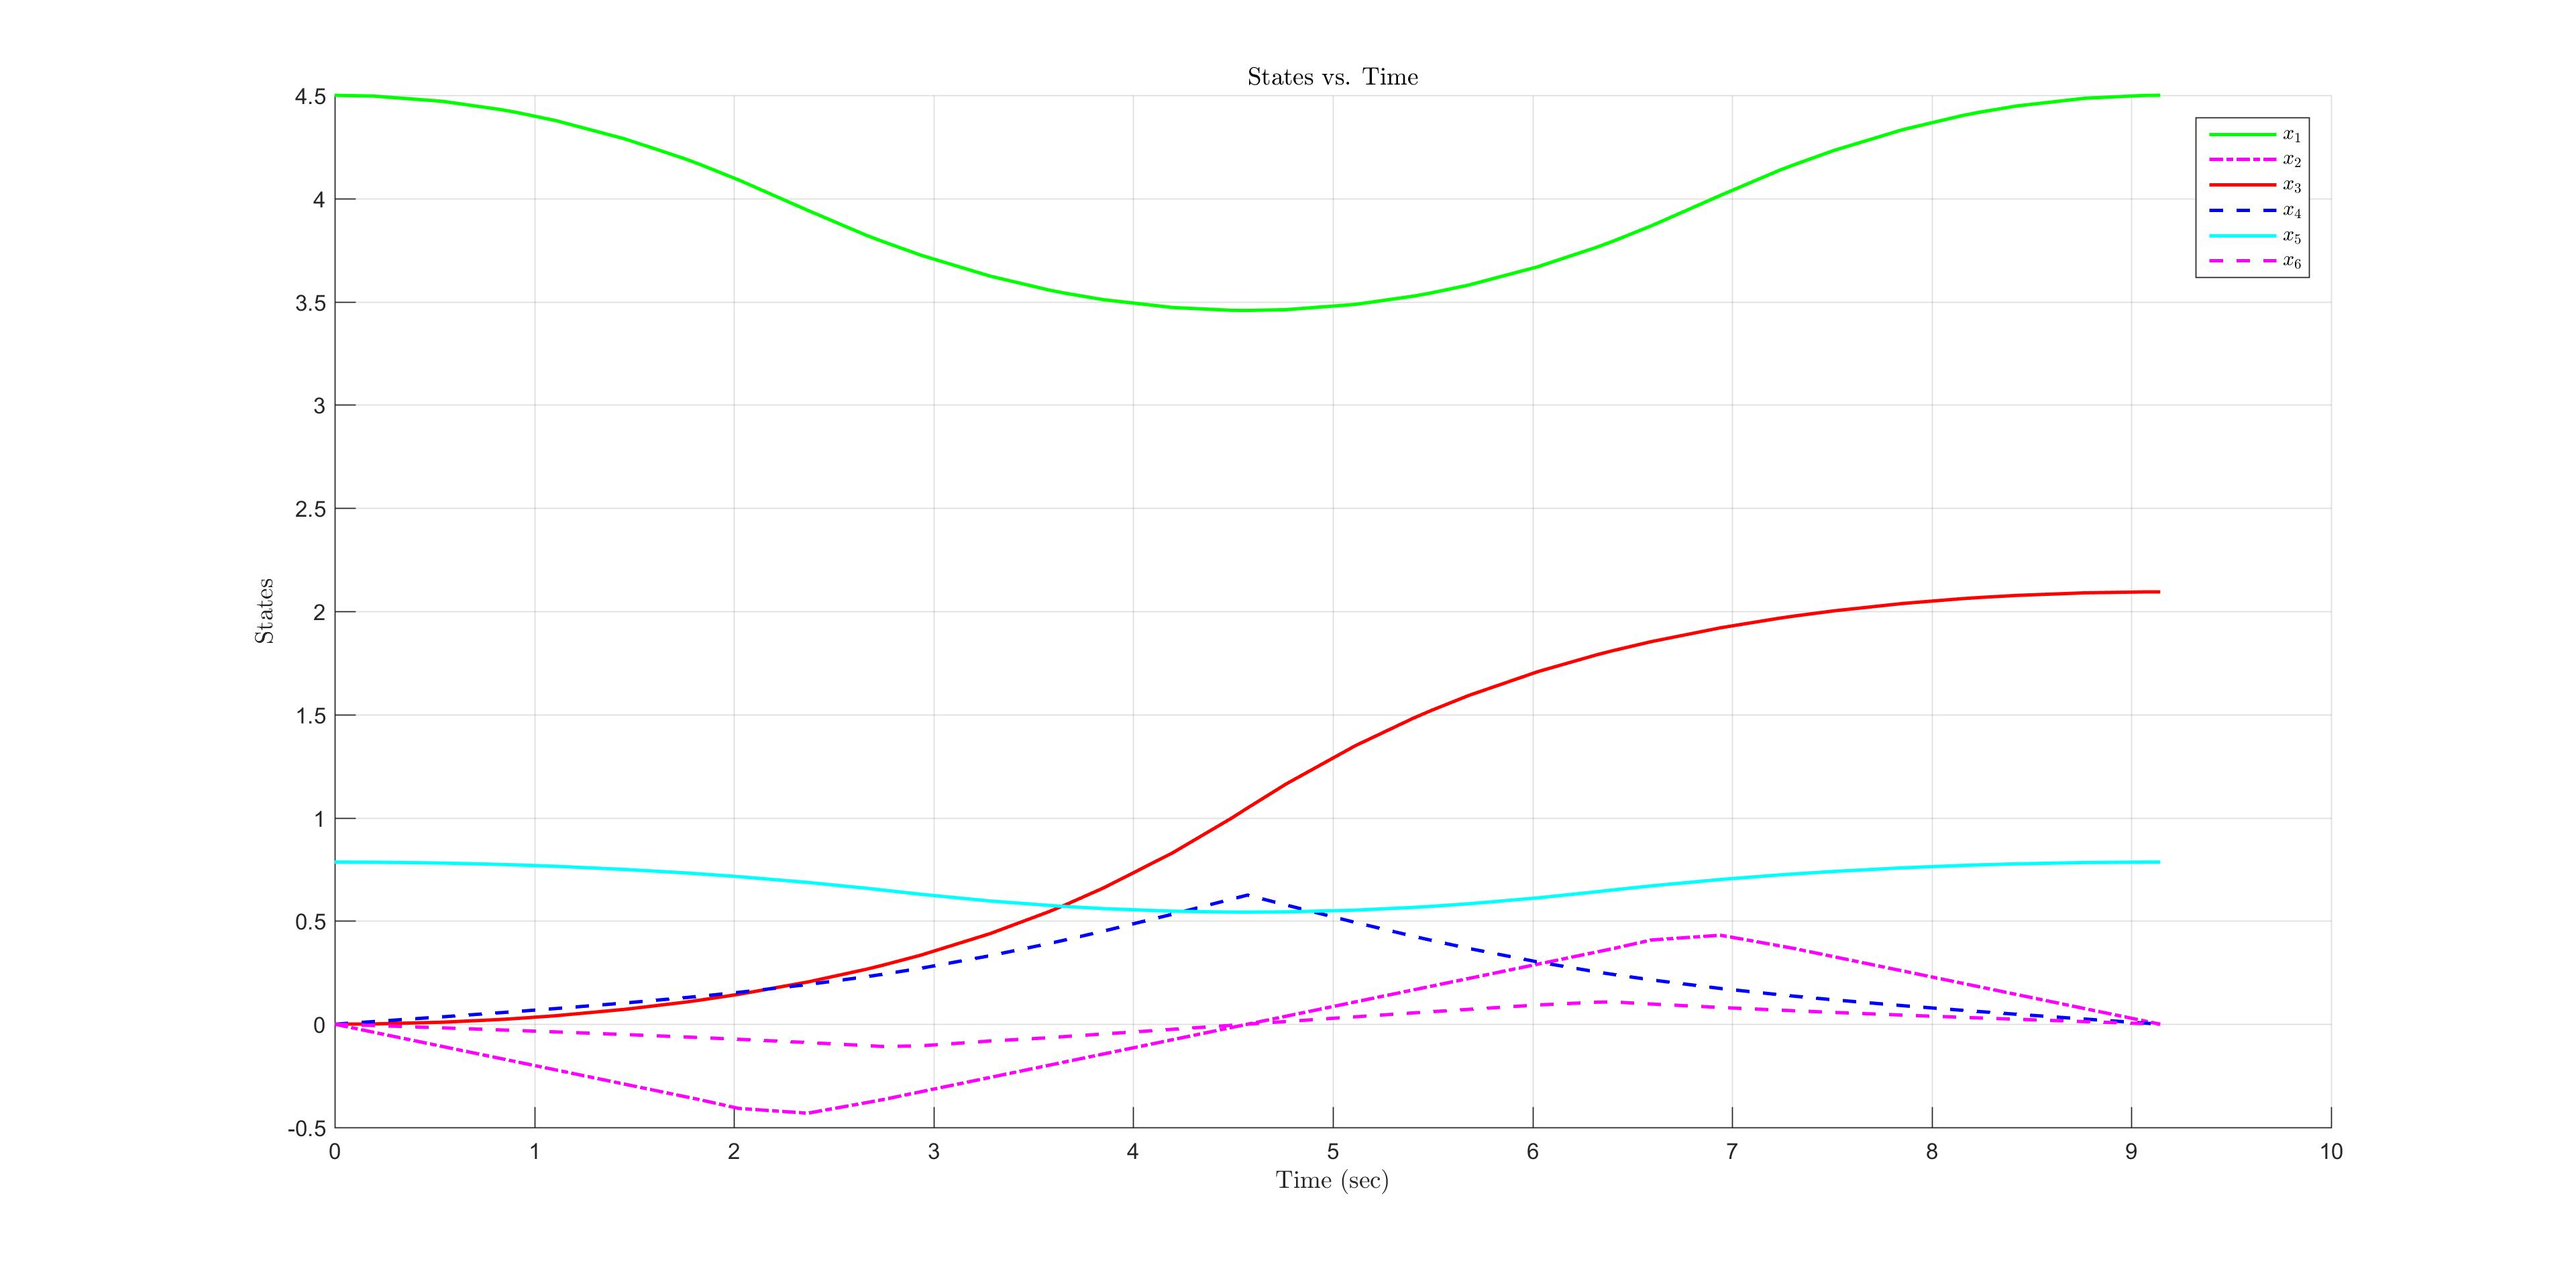
\includegraphics[scale=0.13]{RobotArm_States.jpg}
		\caption{Robot Arm - Collocation - States}
	\end{figure}
	
	\begin{figure}[htpb]
		\centering
		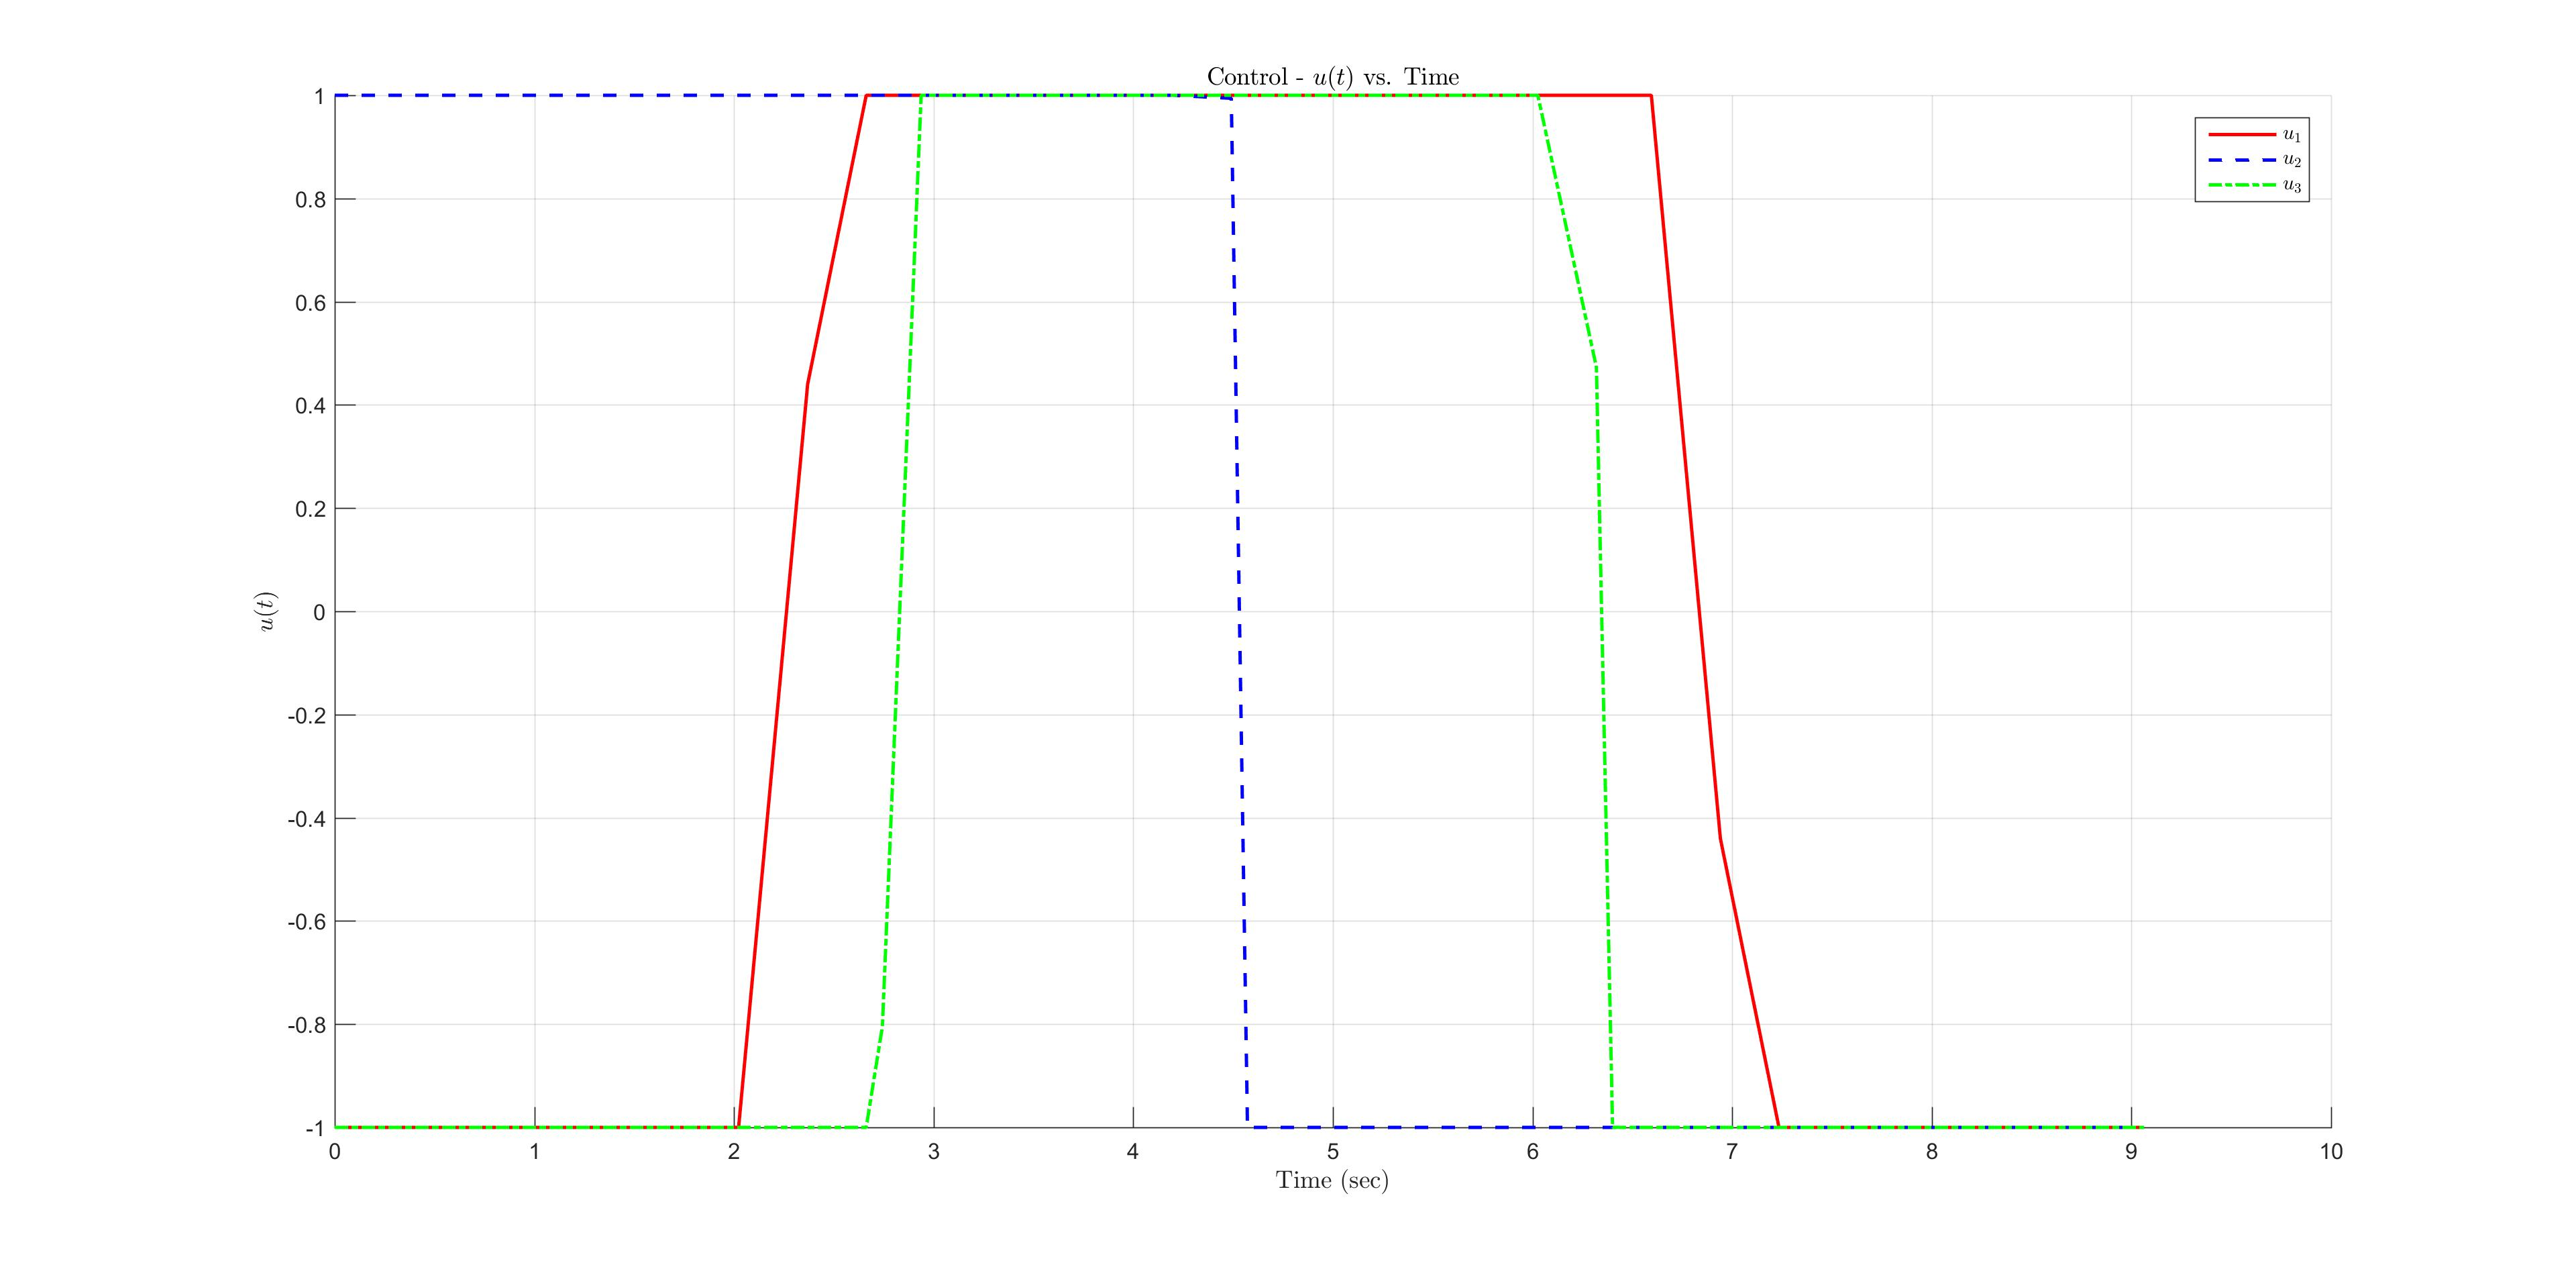
\includegraphics[scale=0.13]{RobotArm_Control.jpg}
		\caption{Robot Arm - Collocation - Controls}
	\end{figure}
	
	\begin{figure}[htpb]
		\centering
		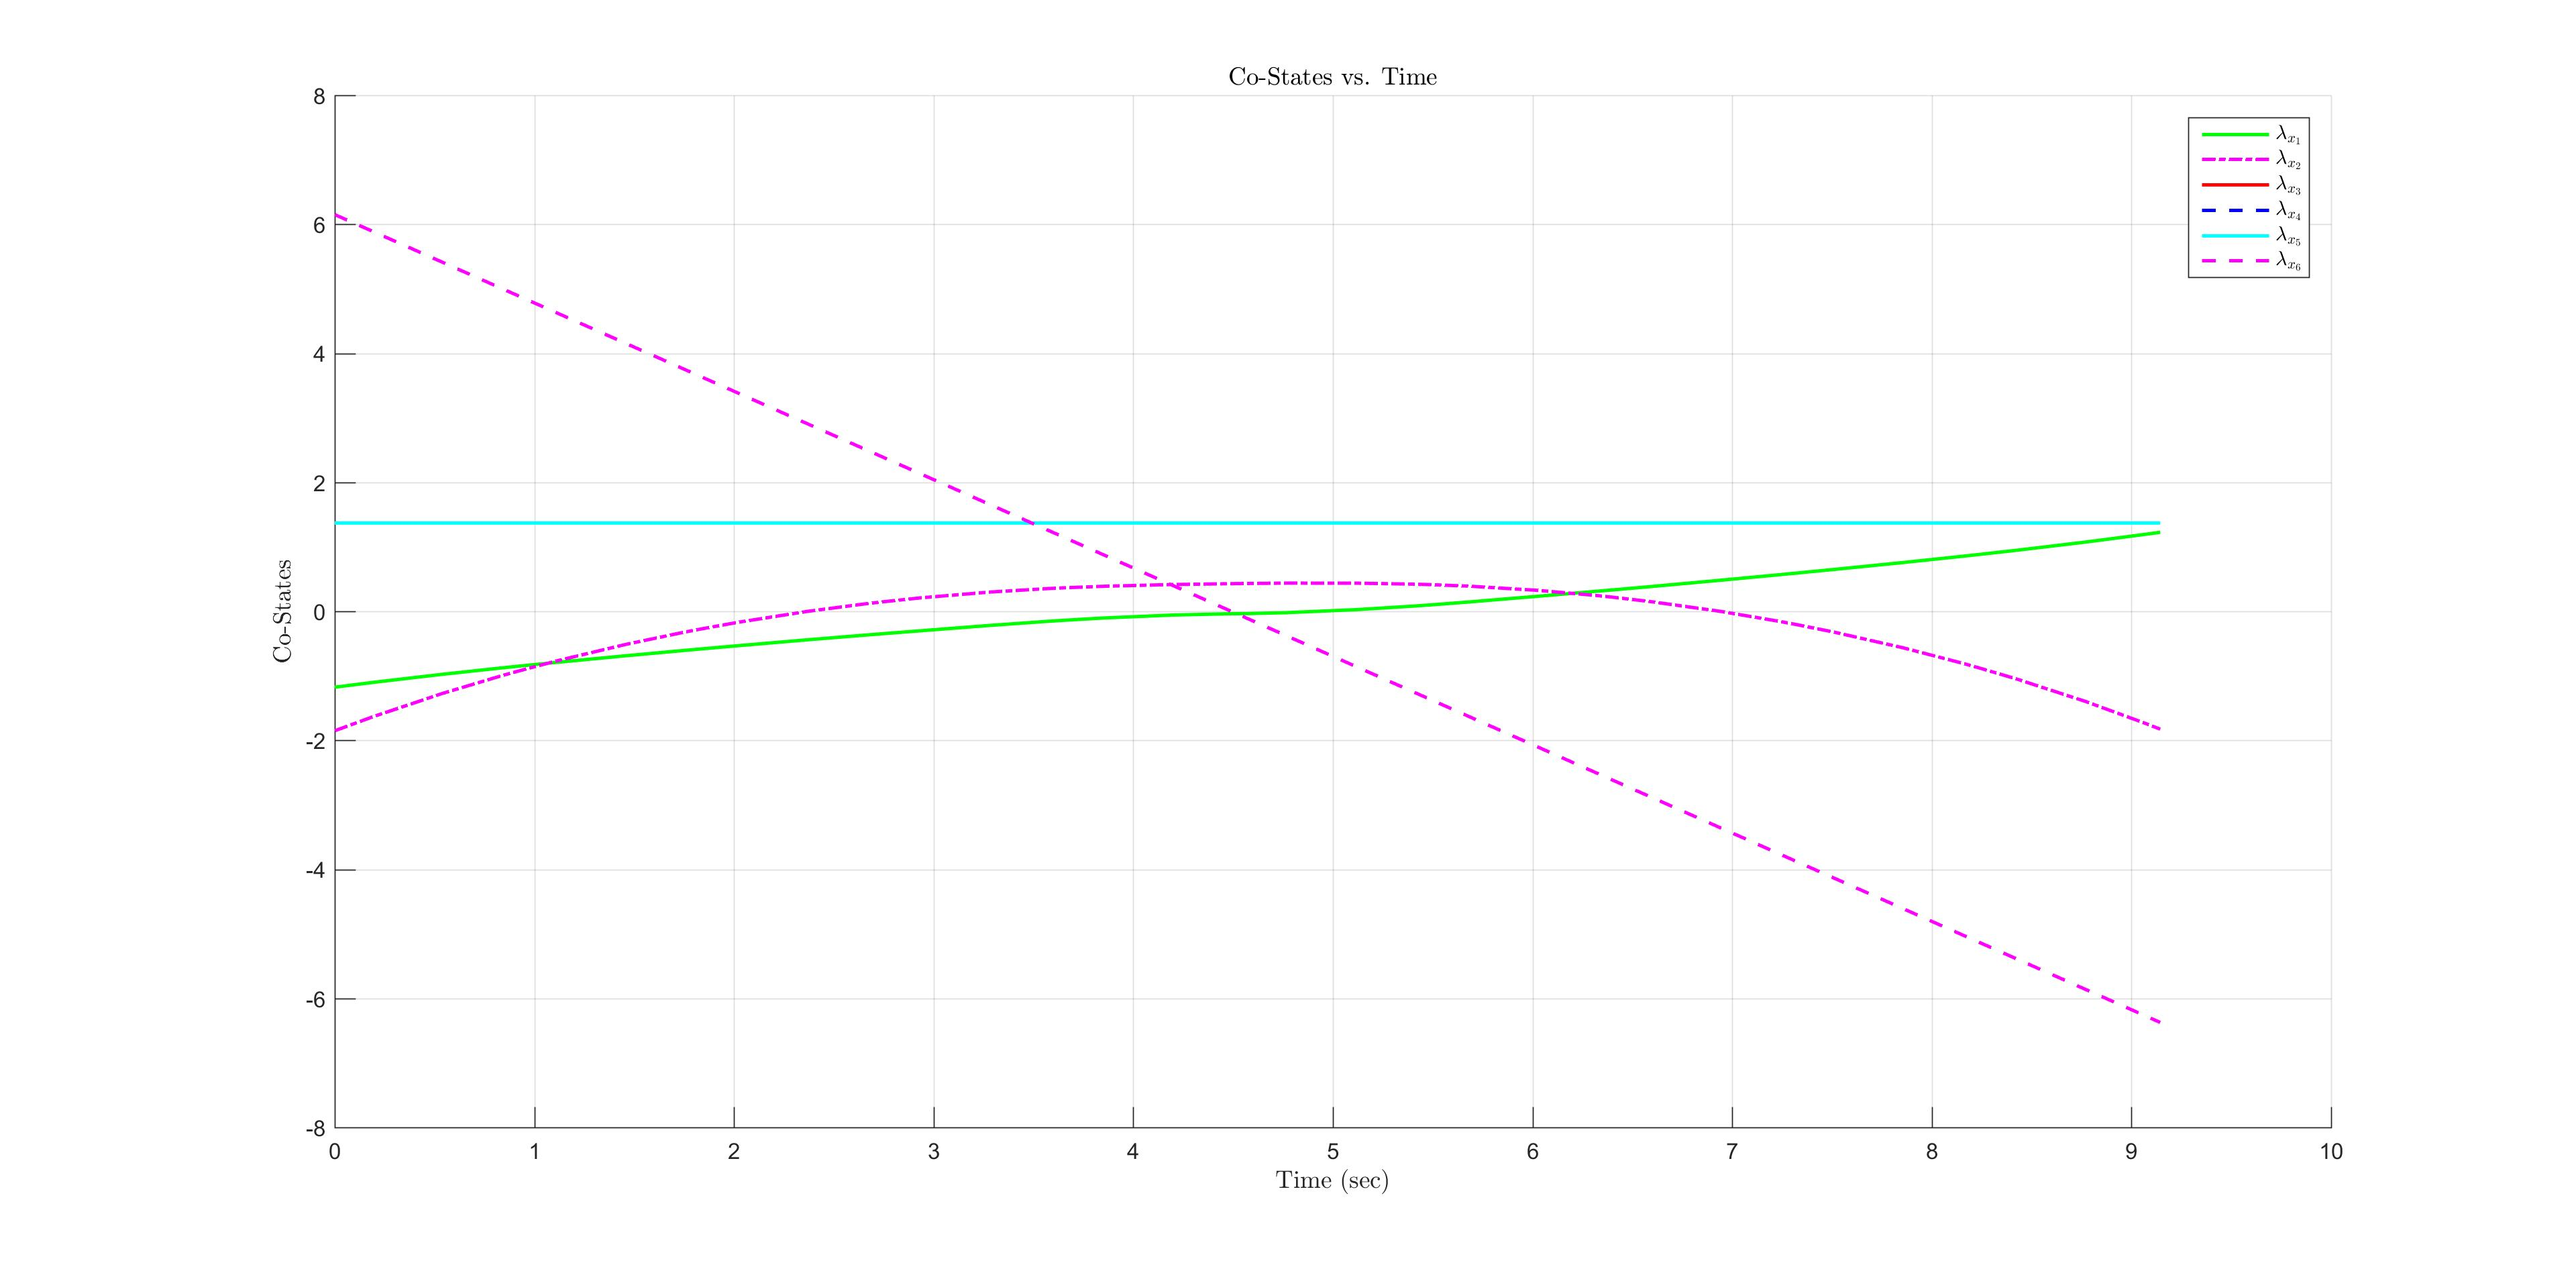
\includegraphics[scale=0.13]{RobotArm_CoStates.jpg}
		\caption{Robot Arm - Collocation - CoStates}
	\end{figure}
	
	\newpage
	
	
	\subsection{Analysis}
	\subsubsection{Proximity of Numerical Solutions to Optimal Solutions}
	The numerical solution found is near to the optimal solution; as, even when the initial conditions are changed the NLP solver gives the same numerical solution. Hence, it shows that this method is robust.
	\subsubsection{Computational Efficiency of the Numerical Method}
	The time taken by this method increases as we increase the degree of the polynomial  and/or the number of mesh intervals. Also, in particular to IPOPT the ma57 solver (0.2856 sec) is faster as compared to the mumps solver (0.3761 sec).
	\subsubsection{Limitation of the Numerical Method}
	The limitation of this numerical method is that the true global minimum is not guaranteed, and we usually find a local optimal solution to our problem. Moreover, this method is not usually robust to changes in the initial guess of the decision variables. Also, for higher accuracy and speed higher order numerical derivatives are required which are complicated to calculate even with algorithmic differentiators.
	\subsubsection{The Ideal Numerical Method}
	An ideal numerical method would be one which is robust to the initial guesses, utilize lower order numerical derivatives and still guarantee global optimum solution.
	
\end{document}












%% Single Figure Environment
\begin{figure}[htpb]
	\centering
	\includegraphics[width=1\columnwidth]{PCN_BaseStation_SoftwareWorkFlow_Basic.pdf}
	\caption{Flywheel Control System}
	\label{fig:FlywheelCSReal}
\end{figure}


